\documentclass[12pt,titlepage]{article}
 
\usepackage[english]{babel}
\usepackage[utf8x]{inputenc}
\usepackage[super]{natbib}
\usepackage[margin=1.4in]{geometry}
\usepackage{amsmath}
\usepackage{graphicx}
\usepackage{amssymb}
\usepackage{enumerate}
\usepackage{mhchem}
\usepackage{units}
\usepackage[title,titletoc,toc]{appendix}
\usepackage{listings}
\usepackage{caption}
\usepackage{subcaption}
\usepackage{hyperref}
\usepackage{tabularx}
\providecommand{\e}[1]{\ensuremath{\times10^{#1}}}
\newcommand{\degree}{\ensuremath{^\circ}}
 
\begin{document}
	\pagenumbering{roman}
	\title{Development of a Spray-On Version of GraphExeter}
	\author{Robert McCorkell}
	\date{April 2013}
	\maketitle
	
	\begin{abstract}
		\setcounter{page}{2}
		Currently the most widespread conductor in optoelectronic applications is Indium Tin Oxide (ITO). Graphexeter, a new material recently developed at Exeter University by intercalating few layer graphene with iron chloride (FeCl$_3$), has a lower sheet resistance than that of ITO whilst being transparent in the visible spectrum and flexible \cite{Khrapach2012a}. Finding a method of manufacturing graphexeter on a large scale could help to revolutionise the optoelectronics industry. 
		
		This project aims to create the material graphexeter in a liquid dispersion for the use of spraying on to substrates. This would allow for cheap manufacturing, and easy deposition of graphexeter on a large scale.
	
		Dispersions of few layer and single layer graphene flakes were exfoliated from flakes of graphite through a process of liquid-phase exfoliation. This process uses ultrasonication to mechanically agitate graphite flakes dispersed in a sodium cholate solution. Highest concentrations of graphene were found from sonicating various types of graphite at 15kHz with a sodium cholate concentration of 0.1mg/ml. Flakes were deposited on to Si/SiO$_2$ substrates by spraying through an airbrush. Flakes were found under an optical microscope using optical interference from the air to graphene/SiO$_2$ interface as an indicator of their location. The presence of graphene was later confirmed through raman spectroscopy of the flakes.
		
		Liquid-phase intercalation was attempted via the same agitation process, with the raman spectra of deposited flakes providing evidence to suggest partial intercalation of iron chloride had been performed. Results are also compared with the vapour-phase intercalation process used in previous studies \cite{Khrapach2012a}. Possible reasons for full intercalation not having occurred are discussed, along with extensions to the project and future work. It is suggested that graphene flakes created through liquid-phase exfoliation are too small in diameter to remain fully intercalated, and until this process is improved to yield graphene flakes with larger diameters, intercalation through liquid or vapour phase may not be possible.
		
	\end{abstract}
	
	\pagenumbering{arabic}
	
	\tableofcontents
	\newpage
	\listoffigures
	\listoftables
	
	\newpage
	\section{Introduction}
	In recent years graphene has gained a large amount of interest due to its remarkable physical and electrical properties. Due to its mechanical flexibility and transparency \cite{Novoselov2011}, there has been much interest in using graphene for optoelectronic applications. However in its pristine form, graphene is not nearly conductive enough to replace the most widespread conductor in optoelectronic applications, indium tin oxide (ITO) \cite{Jo2012,Kumar2010}. In 2012, the Centre for Graphene Science at Exeter University reported the development of a new graphene based material \cite{Khrapach2012a} named graphexeter, which is made up of multiple layers of ferric chloride molecules sandwiched between sheets of graphene. This material's electrical properties outperform that of ITO or any other known carbon-based transparent and flexible conductor currently used in optoelectronics. Even with its enhanced conductivity, graphexeter remains flexible and maintains a similar level of optical transparency to that of pristine graphene.
	
	In order to make graphexeter, graphene flakes were created using mechanical exfoliation of graphite crystals. This process yields flakes with a diameter of the order of microns and a very low level of defects. This process of exfoliation is excellent for experimentation in the laboratory due to its purity, but the size of the resulting flakes leaves a lot to be desired for industrial applications. Thus the goal of this project was to develop graphexeter in a sprayable liquid, allowing for the deposition of a flexible, transparent conductive layer on to almost any surface and at any scale. Such a material could be used to make conductive layers on glass, fabrics or flexible plastics and could help to revolutionise the field of optoelectronics.
	
	In this project flakes of graphene were created using an adapted process of liquid-phase exfoliation \cite{Hernandez2008}, and a process of liquid-phase intercalation was developed in order to make a solution of small graphexeter flakes. This solution was then sprayed onto substrates using an airbrush, and the thickness of flakes and the result of intercalation with ferric chloride was confirmed with the use of raman spectroscopy. 
	
	\newpage
	\section{Background Theory}
	\subsection{Graphene}
	\subsubsection{Structure}
	Graphene is a two dimensional monolayer of carbon atoms arranged in a hexagonal lattice (Figure \ref{fig:graphene}a). It has two atoms per unit cell, and can be viewed as two interpenetrating triangular lattices \cite{Novoselov2011}. The breaking of the hexagonal lattice at the edges of a graphene sheet can be seen to exhibit armchair and zigzag edges shown in Figure \ref{fig:graphene}b \cite{Geim2007}. Graphene sheets are the basic building blocks of graphitic materials of all other dimensionalities, with different constructions making 1D fullerenes, 2D nanotubes, or simply stacked to form 3D graphite \cite{Geim2007}.
	
	\begin{figure}
		\centering
		\includegraphics[width=0.5\textwidth]{figures/graphene.png}
		\caption[The crystal structure of graphene.]{(a) The honeycomb crystal structure of graphene \cite{Novoselov2011}. (b) Scanning electron micrograph of a graphene crystal. Zigzag and armchair edges are represented by blue and red lines respectively \cite{Geim2007}.}
		\label{fig:graphene}
	\end{figure}
	
	Graphene has recently become very popular as a field of research primarily because of its remarkable properties, often superior to other materials. Its charge carriers act as massless Dirac fermions, it is extremely electrically and thermally conductive, very elastic and the worlds strongest material. It is the first known two-dimensional atomic crystal, the thinnest known object and impermeable to other molecules \cite{Novoselov2011}.
	
	Due to the hexagonal symmetry of graphene's lattice, its conduction and valence bands touch at two points in the Brillouin zone, $K$ and $K′$ (referred to as the Dirac Points, Figure \ref{fig:bands}) \cite{CastroNeto2009}. This means that graphene can be regarded as a zero-overlap semimetal with a gapless spectrum and linear dispersion relation \cite{Novoselov2011,Katsnelson2006}.
	
	An integral part of what makes graphene’s electronic properties so unique is the fact that at low energies graphene’s charge carriers act like massless, chiral, Dirac fermions and the chemical potential exactly crosses the Dirac point \cite{Katsnelson2006}. This behaviour mimics the physics of massless fermions in quantum electrodynamics (QED) with the exception that these fermions move at the Fermi velocity $v_f = c/300$ rather than the speed of light \cite{CastroNeto2009,Katsnelson2006}. These massless Dirac fermions are referred to as quasiparticles, which serve as a convenient description of the behaviour of the electrons due to their interaction with the periodic potential of graphene’s hexagonal lattice. They can be viewed as electrons with no rest mass or as neutrinos with an electric charge $e$.\cite{Geim2007}
	
	\begin{figure}
		\centering
		\includegraphics[width=0.7\textwidth]{figures/bands.png}
		\caption[The electronic band structure of graphene.]{The electronic band structure of graphene. Left: energy spectrum  (in units of $t$) for finite values of $t$ and $t'$, with $t=2.7$ eV and $t'=−0.2t$. Right: zoom in of the energy bands close to one of the Dirac points \cite{CastroNeto2009}.}
		\label{fig:bands}
	\end{figure}
	
	\subsubsection{Production}
	One of the most common ways to create graphene in the laboratory is through the micromechanical cleavage technique \cite{Novoselov2004}, sometimes called mechanical exfoliation or the 'scotch tape' technique. This is most likely due to the technique's simplicity, speed and low cost. Graphene produced through mechanical exfoliation also usually has very few defects in comparison to other methods, and therefore allows for graphene's most remarkable properties to be studied in the lab.
	
	In the original form of the mechanical cleavage method a piece of adhesive tape is pressed against a high quality graphite crystal, removing the top layer. The tape is then pressed against a substrate leaving behind thin flakes of graphite typically with a thickness of less than 10nm which attach strongly to the substrate due to van der Waals or capillary forces \cite{Novoselov2004}. Once the flakes have been transferred to a substrate there is a reasonable probability that some of them will be thin enough to be considered graphene. Since the optical transmittance of graphene is very high, it is invisible to the naked eye, so a silicon substrate is commonly used with a 300nm layer of $\text{SiO}_2$. When this layer is in contact with a flake of graphene it causes optical interference when light is shone through. This effect can be viewed with the naked eye as a contrast difference between the graphene flake and the substrate. This means that under white light with the silicon substrate appearing white, graphene flakes will be visible with a faint light blue colour.
	
	\subsubsection{Applications}
	
	With such a wide range of properties, graphene has an equally wide range of applications. Coupled with the ability to make 2D heterostructures out of few layer graphene by adding different chemicals between the layers, and the variety of different production techniques outside of mechanical exfoliation, graphene is likely to form the basis of many technologies in the future.
	
	Table \ref{tab:electronic} lists some of the possible applications for graphene in the field of optoelectronics. Many applications in the field of optoelectronics (such as touch screens, e-paper and OLED displays) require a low sheet resistance and high optical transmittance. Grephene meets these requirements, although the traditionally used Indium Tin Oxide (ITO) still demonstrated slightly better characteristics. Graphene has the advantage over ITO of mechanical flexibility, but more complex graphene based heterostructures are required to compete with the electronic properties of ITO \cite{Novoselov2012}.
	
	\begin{table}
		\begin{scriptsize}	
			\begin{tabularx}{\textwidth}{X X X}
				\hline
				Application & Drivers & Issues to be addressed \\
				\hline
				Touch screen & Graphene has better endurance than benchmark materials & Requires better control of contact resistance, and the sheet resistance needs to be reduced (possibly by doping) \\
				\hline
				E-paper & High transmittance of monolayer graphene could provide visibility &  Requires better control of contact resistance \\
				\hline
				Foldable OLED & Graphene of high electronic quality has a bendability of below 5mm, improved efficiency due to graphene’s work function tunability, and the atomically flat surface of graphene helps to avoid electrical shorts and leakage current & Requires better control of contact resistance, the sheet resistance needs to be reduced, and conformal coverage of three-dimensional structures is needed \\
				\hline
			\end{tabularx}
		\end{scriptsize}
		\caption[Optoelectronics applications of graphene.]{Optoelectronics applications of graphene. \cite{Novoselov2012}}
		\label{tab:electronic}
	\end{table}
	
	\subsection{GraphExeter}
	First developed in 2012 \cite{Khrapach2012a}, graphexeter has an outstandingly high electrical conductivity and optical transparency. With the addition of ferric chloride between its graphene layers, this material shows a record low sheet resistance of $8.8 \Omega/\text{square}$ and an optical transmittance of 84\% in the visible range. These parameters outperform the best values of ITO with a sheet resistance of $10 \Omega/\text{square}$ and an optical transmittance of 85\%. This vastly improves on the best values found in graphene-based materials with typical values of $R_s = 30 \Omega/\text{square}$ and $Tr = 90\%$ for graphene multilayers, and $R_s = 125 \Omega/\text{square}$ and $Tr = 97.7\%$ for chemically doped graphene \cite{Bae2010}. 
	
	Graphexeter is relatively inexpensive to make, and the intercalation of iron chloride (unlike other chemical species that can be introduced between graphene layers) is stable for up to one year. Other stable materials can only be synthesised in the presence of chlorine gas, which is highly toxic. Graphexeter can be produced without the use of chlorine gas using a high temperature two-zone vapour transport method, making it much safer and easier to produce than other materials of its class \cite{Khrapach2012a}.
	  
	\subsubsection{Structure}
	Figure \ref{fig:graphexeter} shows the layered structure of graphexeter. Intercalation of ferric chloride molecules between the layers of pristine few layer graphene causes these layers to decouple and demonstrate properties similar to that of single layer graphene sheets. The ferric chloride molecules act as an acceptor of electrons which lowers the fermi level of the material, increasing the charge carrier concentration of the graphene layers (since charge carriers in graphene are holes), and thus increasing the conductivity.
	
	\begin{figure}
		\centering
		\includegraphics[width=0.5\textwidth]{figures/graphexeter.jpg}
		\caption[The structure of graphene and graphexeter.]{The structure of graphene (left) and graphexeter (right). Ferric chloride molecules intercalate between the layers of graphene, and act as acceptors of electrons.}
		\label{fig:graphexeter}
	\end{figure}
	
	\subsubsection{Production}
	Production of graphexeter flakes starts with micromechanical cleavage of few layer graphene sheets with 3 to 5 layers of graphene on to a $\text{SiO}_2$ substrate in a similar process to that described above for exfoliation of graphene. The substrate and flakes are then placed in a vacuum tube with iron chloride ($\text{FeCl}_3$) where the two-zone vapour transport process takes place \cite{Khrapach2012a,Zhan2004}. The tube is pumped down to a pressure of 2\e{-4}mbar at room temperature for 1 hour to reduce contamination of water molecules, and the FLG and $\text{FeCl}_3$ powder are heated for 7.5 hours at $360^{\circ}$ and $310^{\circ}$ respectively in separate zones. This causes the $\text{FeCl}_3$ to sublimate and diffuse to the higher temperature zone where intercalation takes place. Some situations can cause deintercalation to take place on some layers, for example rinsing in acetone during lift-off of the substrate. However graphexeter is stable to most typical stimuli and has been shown to be stable in air for up to one year \cite{Khrapach2012a}.
	
	\subsection{Liquid-Phase Exfoliation and Sodium Cholate}
	In order to produce graphene in the form of a sprayable liquid, a method of fabrication called liquid-phase exfoliation was used. This process was chosen because of its low cost (figure \ref{fig:cost}) and high yield of graphene flakes in dispersion which is perfect for later spraying on to substrates \cite{De2010,Lotya2009a}. In this process graphite flakes are dispersed in a liquid medium, and agitated by an external force to help overcome the van der Waals forces between the layers of graphite. This external force is provided by an ultrasonication bath which uses ultrasound waves to generate the mechanical agitation \cite{Hasan2010}.
	
	\begin{figure}
		\centering
		\includegraphics[width=0.6\textwidth]{figures/cost.png}
		\caption[Methods of mass production of graphene.]{Several methods of mass production of graphene. Methods cover a range of costs, often with a reduction in quality at low cost \cite{Novoselov2012}.}
		\label{fig:cost}
	\end{figure}
	
	The energy required for exfoliation to take place in a liquid is at a minimum when the enthalpy of mixing of the graphene in solution is close to zero \cite{ONeill2011}. This requires the liquid to be a solvent with surface tension approaching $40 \text{mJ/m}^2$, which is satisfied by solvents with a boiling point close to $200^{\circ}$C \cite{Coleman2008a,Lee2009}. However exfoliation of graphene can also take place in a aqueous-surfactant solution, for example a solution of sodium cholate (NaC) \cite{Lotya2009a,Yumin2011a}. 
	
	Sodium cholate has amphiphilic properties whereby its molecules possess both hydrophobic and hydrophilic parts. In water, these molecules align themselves into aggregates where the hydrophilic heads form the water facing part of the aggregate and the hydrophobic tails form the core of the aggregate, shielded from contact with the water. This property of sodium cholate enables it to form a stable encapsulation layer around graphene sheets and stabilise the hydrophobic graphene surfaces \cite{Wang2009} from reforming back together to form bulk graphite. This process provides a low degree of agglomeration, and a high yield of few layer graphene flakes dispersed in the solution \cite{De2010}.
	
	\subsection{Liquid-Phase Intercalation}
	Using a similar ultrasonication process, this project will investigate how the addition of heating to sonication could also allow for ferric chloride molecules to intercalate between the layers of graphene in few layer graphene flakes.
	
	Once few layer graphene flakes have been exfoliated from bulk graphite, ferric chloride molecules will require additional energy to overcome the surface energy of the flakes and intercalate between the graphene layers. The process of intercalation is dependant on constraints associated with intercalant size and bonding distances, and increasing the temperature can help this reaction to take place \cite{Khrapach2012a}. This could be provided by heating the dispersion in addition to sonication, and therefore the highest temperature provided by the available equipment will be used. In most cases this temperature will be limited by the heating ability of the sonication bath, but it may be possible to order new equipment that can heat dispersions to temperatures an order of magnitude higher than a sonication bath, whilst gently mixing them with a magnetic stirrer.
	%Why would this work?
	
	\subsection{Raman Spectroscopy}
	In order to probe the thickness of graphene flakes, and therefore determine the number of graphene layers present in a flake, raman spectroscopy is used. This has a distinct advantage over methods that purely measure the thickness of a sample like Atomic Force Microscopy (AFM) because in this project multiple small flakes will be sprayed on to a substrate, some resting on others and overlapping. AFM would simply measure the thickness of the sample regardless of how many flakes are present, whereas the shape of the peaks present in the raman spectrum of graphite gives information on the physical properties of the flakes.
	
	A raman spectrometer probes a sample with laser light (in this case 532nm at room temperature and pressure), and measures the changes in wavelength received when the light is reflected back due to phonon interactions. Different types of interaction cause different peaks to appear on a plot of arbitrary counts against inverse wavelength. Figure \ref{fig:raman} (top) shows part of the typical raman spectrum of few layer graphene. Here we see the G peak (1580cm$^{-1}$) which is due to phonon interactions caused by stretching across the carbon-carbon bonds of the hexagonal lattice of a graphene sheet. This peak increases in intensity as more layers are added since each layer has more carbon bonds present for phonon interactions to take place. 
	
	The D peak (or defect peak at 1350cm$^{-1}$) in graphite's raman spectrum is caused by a more complex interaction involving an electron being excited into the conduction band and being scattered by a phonon into an adjacent Brillouin zone. For the electron to decay again, there must be a hole for it to decay into, and this can be provided if there are defects or broken benzene rings in the lattice \cite{Casiraghi2008,Casiraghi2007a}. Therefore the intensity of the D peak can be used as a measure of the defects in the sample. The 2D peak (1700cm$^{-1}$) seen in figure \ref{fig:raman} is the second order of this interaction. This represents an electron scattering into an adjacent Brillouin zone, and then being scattered back again by another phonon only to decay into its original hole. The 2D peak of single layer graphene can be seen as a single peak, but as more layers are added the peak becomes less symmetrical and is made up of multiple smaller peaks. This is because the band structure of multilayer graphene is more complex and therefore there are multiple ways for the 2D process to occur, represented by slightly different wavelengths on the raman spectrum (figure \ref{fig:bilayer} shows the band structure of bilayer graphene as an example) \cite{Ferrari2006,Ferrari2007,Vidano1981}.
	
	\begin{figure}
		\centering
		\begin{minipage}[b]{.45\linewidth}
			\centering
			\includegraphics[width=0.6\textwidth]{figures/raman.png}
			\caption[Typical raman spectra of graphene and graphexeter.]{(Top) part of the typical raman spectrum of few layer pristine graphene. (Middle) part of the typical raman spectrum of graphene intercalated with ferric chloride to create graphexeter. Splitting of the G-peak into $\text{G}_1$ and $\text{G}_2$ is caused by the number of adjacent layers of ferric chloride to a graphene sheet (bottom) \cite{Khrapach2012a}. }
			\label{fig:raman}
		\end{minipage}
		\begin{minipage}[b]{0.45\linewidth}
			\centering
			\includegraphics[width=0.6\textwidth]{figures/bilayer.png}
			\caption[The electronic band structure of bilayer graphene.]{The electronic band structure of bilayer graphene in the vicinity of the $K$ point. More complex band structures like these allow for the raman 2D interaction to take place multiple ways \cite{Novoselov2011}.}
			\label{fig:bilayer}
		\end{minipage}
	\end{figure}
	
	Once intercalation has taken place with ferric chloride between graphene sheets we expect to see a change in the G peak of the raman spectra (figure \ref{fig:raman}, middle). The layers of ferric chloride adjacent to sheets of graphene increase the charge carrier concentration of the graphene, decreasing the fermi level and therefore changing the energies of the phonon interactions across the carbon bonds. This causes the G peak to move to G$_1$ (1612cm$^{-1}$) if one adjacent ferric chloride layer is present, and mover further to G$_2$ (1625cm$^{-1}$) if two adjacent ferric chloride layers are present (figure \ref{fig:raman}, bottom) \cite{Khrapach2012a}.
	
	Another consequence of intercalation is the fact that the 2D peak becomes symmetrical regardless of the number of layers (up to $\sim$5 layers). This is because the ferric chloride layers decouple the graphene layers from each other, causing them to behave like single layer graphene within the multilayered structure of graphexeter. These properties of graphexeter's raman spectrum serve as a clear indication of the occurrence of intercalation on a graphene flake \cite{Khrapach2012a}.
	
	\newpage
	\section{Experimental Techniques and Methods}
		All work was carried out inside a ventilated cleanroom with full body cleanroom suits, hoods and gloves to prevent contamination of samples. When spraying solutions containing iron chloride face masks were worn to prevent inhalation. Before use, all equipment was thoroughly cleaned by sonicating in acetone at 15kHz for 1 hour, then sonicating in isopropanol alcohol (IPA) for 1 hour and finally evaporating residual IPA with a nitrogen spray. All water used in experiments was deionized. 
		
	\subsection{Liquid-Phase Exfoliation}
	
	Liquid phase exfoliation was performed in a Fisher Scientific sonication bath at 15 kHz. Sodium cholate solutions were mixed with a concentration of $0.1\pm 0.01$mg/ml using previous studies as a guide \cite{De2010}. In order to aid in measuring such small concentrations a solution with $1\pm 0.01$mg/ml of sodium cholate was mixed in 100ml using a magnetic stirrer at 5000rpm for a minimum of 6 hours (usually left overnight). 10ml of this 10x concentration solution was then filled back up to 100ml with deionized water (DI-water) and a magnetic stirrer was used for a similar amount of time to create a solution of the desired concentration.
	
	$3\pm 0.1$g of Graphite flakes were then added to the 100ml solution and shaken briefly to disperse them. Graphite sourced from China, England, Madagascar, Sri Lanka, Korea and Washington were tested.
	
	\subsubsection{Sonication}
	These dispersions were then placed in a sonication bath and sonicated for a variety of times with no extra heating. Sonications were performed on sealed bottles to prevent evaporation since parafilm stretched over a bottle was found to split over time. The energy provided by sonication is reliant on factors such as water level, position on the bath, geometry of the flasks, and volume of the dispersion \cite{ONeill2011}. These factors were kept mostly constant to minimise these effects. For example sonication bottles were held in a plastic frame to stop them from moving, and the baths were checked regularly to make sure the water was topped up to the maximum level. Smaller vials were held inside a thin layer of foam to keep them upright at the surface of the water. Sonication times tested were 2, 4, 6, 20, 30 40 and 50 hours.
	
	\subsubsection{Centrifugation and Filtration}
	The top 40ml of the resulting solution was then pipetted into a 50ml vial and centrifuged in a  Heraeus Megafuge 11 centrifuge for 90 minutes at various speeds. This process acts as accelerated sedimentation, and removes the thicker graphitic flakes from the thinner flakes of few layer graphene \cite{Hasan2010}. It was found that similar results could be achieved with smaller centrifuge times, so this was reduced to 10 minutes towards the end of the project. Centrifuge speeds tested were 2500, 3000 and 4000 rpm. 
	
	After centrifugation the top 75\% of supernatant (30ml) was pipetted out of the vial and stored for later use. Vacuum filtration was also attempted to remove larger flakes using the most porous filters that were available ($0.45\mu$m millipore) but this was found to filter out almost all remaining flakes and was not pursued further.
	
	\subsubsection{Deposition}
	Substrates of silicon and a 300nm layer of SiO$_2$ were cut to 1cm squares from a larger wafer using a diamond tipped scriber. All cuts were made parallel to atomic bonds using markings on the wafer. These substrates were then cleaned using normal cleaning procedures mention above. To aid in the deposition process, some substrates were saturated in water for 1 week before deposition took place.
	
	Two methods of deposition were tested. Dispersions were drop coated using a pipette onto substrates and left to dry in air. Accelerated drying was also tested in an oven set to $50^{\circ}$C, but this was found to cause excessive oxidisation of flakes and was not pursued. When water dried from drop coating, it was found that droplets would dry from the outside in, carrying all flakes within the droplet and releasing them together in the centre. This made it impossible to identify single thin graphene flakes so this method was deemed unsuitable.
	
	The other method of deposition was spraying \cite{Pham2010}, the core method of the project. Here a modelling airbrush was used for its precision and fine spray. An example of which is shown in figure \ref{fig:airbrush}. This device takes liquid in from a reservoir at its top, and gas (in this case nitrogen at 1 bar) in a tube at the bottom. Gas pressure is controlled by pushing down on a lever, and pulling back on the same lever pulls back a pin in the tip of the device. This provides a small amount of space for the liquid and nitrogen to escape in the form of a fine spray. This spray forms many small droplets on the substrate unlike the large droplets made from drop coating.
	
	\begin{figure}
		\centering
		\includegraphics[width=0.5\textwidth]{figures/airbrush.jpg}
		\caption[The modelling airbrush used for deposition.]{An example of the modelling airbrush used for deposition. Pushing the lever down controls gas pressure, and pulling the lever back controls liquid flow.}
		\label{fig:airbrush}
	\end{figure}
	
	Initially a similar problem to drop coating was observed but on a smaller scale. Flakes were pushed to the centre of each small droplet where they would overlap, making identification impossible. This was solved by heating the substrate to $120^{\circ}$C on a hotplate before spraying which caused the water to immediately evaporate on contact, and dropping the individual flakes.
	
	Deposition leaves behind a large amount of sodium cholate, appearing under the microscope as a multicoloured residue. This can be confusing when searching for a slight optical contrast signifying a graphene flake on the substrate. It was found that by soaking the substrates for 5 minutes in water, most of this residue would wash away. To improve coverage of flakes on the substrate multiple coatings were tested (up to 10). Simply spraying multiple coats and soaking the substrate in water between coats to remove NaC residue was also tried. A high density of flakes on the substrate is desirable because this would allow for flakes to touch each other, creating a continuous electrical channel across the substrate \cite{De2010}. Therefore achieving this would give us a large-scale sprayable conductor, and allow for electrical measurements to be made on a macroscopic scale without the use of electron beam lithography.
		
	\subsection{Liquid-Phase Intercalation}
	The process developed for this project of liquid-phase intercalation is very similar to that of liquid-phase exfoliation. The goal is to create intercalated graphexeter in the liquid-phase before deposition onto a substrate, so no further processing is required on the substrate. This should allow for many different types of substrates to be used like plastics or delicate fabrics.
	
	Iron chloride powder is mixed with a given dispersion of graphene and placed in a sealed bottle for sonication. Sonication takes place at 15kHz as before, with extra heating at $80^{\circ}$C. Concentrations of FeCl$_3$ of 1, 2 and 5 g/100ml and sonication times of 5 - 13 hours in intervals of 2 hours and, 17 - 29 hours in intervals of 4 hours were tested.
	
	It was also theorised that if the processes of LPE and LPI were very similar, it might be possible to perform them simultaneously with few layer graphene sheets breaking apart and being intercalated at the same time. This was tested by mixing iron chloride powder with graphite flakes and the same sodium cholate solution as before, and sonicating at $80^{\circ}$C. Sonication times tested were 10, 20, 30 and 40 hours with 2g/100ml FeCl$_3$. This was done by stopping the sonication at the given times, taking small samples of 2.5ml with a pipette and continuing the sonication afterwards. A control bottle of just graphite and sodium cholate solution was also sonicated with samples being taken out and measured at the same time.
	
	Once the desired number of hours of sonication have taken place, samples were pipetted into an airbrush and sprayed onto a heated substrate as before.
	
	\subsection{Identification and Raman Spectroscopy}
	Once samples had been sprayed onto a substrate, the substrates were placed in a Renishaw raman spectrometer for measurement. The process of measurement involves first calibrating the machine with a sample of silicon, since silicon provides a very clear peak in the raman spectrum at $520\text{cm}^{-1}$. The machine can then compare the expected location of this peak to the data received and calibrate for future measurements.
	
	Points of interest are then found on the sample under an optical microscope, and then focusing the laser on that point. Once the laser is in position a scan is performed over a 20 second period between $300\text{cm}^{-1}$ and $3500\text{cm}^{-1}$ as the expected peaks are between these values. Points of interest might include locations of contrast from the majority of the substrates, locations of different colour or clear shapes on the substrate.
	
	One process of determining the thickness of few layer graphene measured by the raman spectrometer is to calculate the ratio $I_G/I_{Si}$ if the intensity of the G peak to the silicon peak. Since the G peak intensity increases as the number of graphene layers increases, and the intensity of the silicon peak decreases, this ratio can serve as an indication of the number of layers present in a flake when compared to past data \cite{Khrapach2012a}.
	
	The raman spectrometer outputs data as a simple columnated text file, so a MATLAB script was written by me to process this data. The script calculates the $I_G/I_{Si}$ ratio and displays spectra along with zooms of the silicon peak, G and 2D peaks for viewing. This script can be found in Appendix \ref{app:ramanratio}, and an example of its output can be seen in figure \ref{fig:mad-sample}.
	
	\subsection{Electrical Measurements}
	To perform electrical measurements silver paint is painted on the substrate using toothpicks in a four-point probe configuration. A four-point probe is a method of measuring the potential difference across the sample resulting from an applied current without taking into account the resistivity of the probe contacts. In this case we can use it to measure the resistance across our sample irrespective of the resistance of the silver paint. Figure \ref{fig:probe} shows an example layout of this method. A current is applied across the outer terminals, and the potential difference is measured across terminals 1 and 2. \cite{Smits1958}
	
	\begin{figure}
		\centering
		\includegraphics[width=0.5\textwidth]{figures/probe.png}
		\caption[The four-point probe.]{An example layout of the four-point probe. A current is applied across the outer terminals, and the potential difference is measured across terminals 1 and 2 \cite{Smits1958}.}
		\label{fig:probe}
	\end{figure}

	Measurements of current were attempted on sprayed substrates using a lock-in amplifier with an applied potential difference of 10mV using a potential divider created for the purpose in the lab. The lowest resistance calculated from multiple samples tested was $10\text{M}\Omega$, which is order of magnitudes higher than expected. It was determined that this was due to the density of flakes on the substrate not being high enough for a continuous conduction path to be possible between the contacts. Since this was not achieved in the given time, this is an example of future work that can be done on the project.
	
	Electrical characterisation of single flakes would be possible using electron-beam lithography to etch contacts on to a flake. Electron beam lithography typically has resolutions down to a few nanometres which is easily small enough since graphene flakes exfoliated in this project had diameters of $\sim 1\mu$m. Unfortunately there was not enough time in this project to perform electron beam lithography on flakes so this is another example of	 future work.
	
	\newpage
	\section{Results and Analysis}
	\subsection{Liquid-Phase Exfoliation}
	As sonication times of liquid-phase exfoliation increased the dispersions were observed to become darker in colour. This suggests at least lateral breakup of flakes had occurred, dispersing the graphite more evenly in the fluid.
	
	%Pictures - Sonication times causing darker samples.
	
	Centrifugation of dispersions successfully caused sedimentation of larger flakes to the bottom of vials (figure \ref{fig:centrifuge}), making identification of thin graphene flakes much easier on the substrate (figure \ref{fig:centrifuge-substrate}). As the centrifuge speed was increased the colour of dispersions was observed to become lighter suggesting that an increased speed causes more flakes to be pushed to the bottom of the vial as expected. For highest sonication times (50 hours) no change was seen in the colour of samples after centrifugation of speeds up to 4000rpm. This is likely due to the dispersion being made up of a high proportion of thinner flakes that require higher centrifuge speeds for sedimentation to occur. Centrifuge speeds higher than 4000rpm were not possible with the equipment available.
	
	\begin{figure}
		\centering
		\includegraphics[width=0.5\textwidth]{figures/centrifuge.png}
		\caption[The effects of centrifugation.]{A sample of English graphite sonicated for 40 hours before and after centrifugation at 3000rpm for 10 minutes. Sedimentation occurs for the largest flakes at the bottom of the vial leaving thinner flakes dispersed in the supernatant.}
		\label{fig:centrifuge}
	\end{figure}
	
	\begin{figure}
		\centering
		\includegraphics[width=1\textwidth]{figures/centrifuge-substrate.png}
		\caption[The effects of centrifugation after deposition.]{Madagascan graphite sonicated for 40 hours (a) Before and (b) after centrifugation at 3000rpm. Centrifugation removes many of the larger graphite flakes, leaving the thin flakes much easier to identify.}
		\label{fig:centrifuge-substrate}
	\end{figure}
	
	%Picture - samples get clearer as centrifuge goes faster
	
	Vacuum filtration of dispersions to remove more large flakes was found to remove almost all flakes from dispersions using the most porous filters available ($0.45\mu$m millipore). Liquid output from the filter was almost clear, and very few flakes were found upon deposition (figure \ref{fig:filter}). 
	
	\begin{figure}
		\centering
		\includegraphics[width=1\textwidth]{figures/filter.png}
		\caption[The effects of vacuum filtration.]{Chinese graphite sonicated for 20 hours, sprayed onto  substrate and left to dry in air. (a) After filtration using $0.45\mu$m millipore filter paper. Very few flakes are present. (b) Before filtration. Many more flakes are visible that have been removed in the filtration process.}
		\label{fig:filter}
	\end{figure}
	
	Spray coating was deemed more effective than drop coating for depositing flakes. Drop coating with a pipette caused flakes to be deposited at the centre of a droplet during drying, whereas spray coating covered the substrate more evenly (figure \ref{fig:pipette}). 
	
	\begin{figure}
		\centering
		\includegraphics[width=1\textwidth]{figures/pipette-vs-spray.png}
		\caption[Comparison of drop coating and spray coating.]{(a) Drop coating of Chinese graphite sonicated for 6 hours. Graphite flakes are deposited in the centre of the droplet after it dries (top right). (b) Spray coating of Chinese graphite sonicating for 40 hours. Spray coating allows for a more even spread of flakes over the substrate.}
		\label{fig:pipette}
	\end{figure}
	
	Heating the substrate also allowed for a more even distribution of flakes since droplets evaporated as soon as they came into contact with the substrates, immediately dropping any flakes in the dispersion on to the substrate. Graphene deposited by this method can be seen in figure \ref{fig:soaking}. Drying in an oven at $50^{\circ}$C still caused graphite to be deposited in the centre of a droplet and caused oxidisation of the graphite as shown in figure \ref{fig:oven}.
	
	\begin{figure}
		\centering
		\includegraphics[width=0.6\textwidth]{figures/oven.jpg}
		\caption[Oxidisation of graphite after oven drying.]{Chinese graphite sonicated for 40 hours and pipetted onto a substrate. Oven drying at $50^{\circ}$C caused oxidisation of the graphite and did not prevent graphite flakes from being deposited in the same place in the middle of a droplet.}
		\label{fig:oven}
	\end{figure}
	
	Once deposition had been performed, a large amount of sodium cholate residue was often left behind. This made optical identification of graphene flakes in the raman spectrometer difficult. Samples were soaked in water for 5 minutes to remove most of this residue. Figure \ref{fig:soaking} shows the sodium cholate residue before and after soaking a sample.
	
	\begin{figure}
		\centering
		\includegraphics[width=1\textwidth]{figures/soaking.png}
		\caption[Comparison for soaking of samples to remove NaC residue.]{Madagascan graphite sonicated for 40 hours, centrifuged at 3000rpm and sprayed on to a substrate. (a) Before soaking. The coloured areas show sodium cholate residue making the blue graphene flakes hard to see. (b) After soaking in water for 5 minutes. Much of the sodium cholate residue is gone leaving behind clear flakes of graphene.}
		\label{fig:soaking}
	\end{figure}
	
	In order to improve the density of flakes deposited on a substrate, the deposition of multiple spray coats was tested. In order to allow contact between flakes of graphene for electrical conduction the substrates were soaked in water between coats to remove NaC residue between layers. A comparison of visible flakes for the number of coats sprayed can be seen in figure \ref{fig:coats}.
	
	\begin{figure}
		\centering
		\includegraphics[width=1\textwidth]{figures/coats.png}
		\caption[Comparison of flake density for number of spray coats.]{English graphite sonicated for 40 hours, centrifuged at 4000rpm and sprayed on to a substrate. (a) 1 coat. (b) 5 coats. (c) 10 coats. The substrate was soaked in water for 5 minutes between coats to remove sodium cholate residue.}
		\label{fig:coats}
	\end{figure}
	
	As sonication time was increased, a decrease in flake diameter was observed in all types of samples as illustrated in figure \ref{fig:sonication-size}. Increased sonication time also resulted in the flakes having fewer layers. As sonication time was increased fewer flakes were found that gave a raman spectrum similar to that expected for thick graphite (having a G peak with a larger intensity than the silicon peak), and the number of flakes observed with raman spectra similar to that expected for few layer graphene increased (with the intensity of the silicon peak much greater than the G peak, yet the G and 2D peaks still present).

	\begin{figure}
		\centering
		\includegraphics[width=1\textwidth]{figures/sonication.png}
		\caption[Comparison of sonication times on flake diameter.]{Deposition of flakes by spray coating from sonication of Madagascan graphite sonicated for (a) 2, (b) 4, (c) 6, (d) 30 and (e) 40 hours. As sonication time increases the diameter of flakes decreases.}
		\label{fig:sonication-size}
	\end{figure}

	%Graph? - Average flake size vs sonication time.
	
	However, some types of graphite were found to be more resilient to sonication, giving a lower yield of thin graphene flakes in comparison to other graphite types for the same sonication time. For example Chinese graphite was found much fewer graphene flakes, and thicker flakes in general than Madagascan graphite for the same sonication time as shown in figure \ref{fig:flake-type}.

	\begin{figure}
		\centering
		\includegraphics[width=1\textwidth]{figures/flake-type.png}
		\caption[Comparison of graphite sources with the same sonication time.]{(a) Chinese,(b) Korean, (c) Madagascan, (d) Sri Lankan, (e) Washington and (f) English graphite sonicated for 40 hours and sprayed on to a substrate. Different types of graphite on average yield different sizes of flakes for the same sonication time. They also give different yields of thin graphene, the most of which can be seen with Madagascan graphite. Blue flakes are usually thin graphene flakes, which are much easier seen after centrifugation, as in figure \ref{fig:centrifuge-substrate}.}
		\label{fig:flake-type}
	\end{figure}
		
	Raman spectra with the clearest peaks resembling the expected raman spectrum of graphene came from samples of Madagascan graphite sonicated for 40 hours, centrifuged at 3000rpm for 90 minutes, sprayed onto a substrate heated to $120^{\circ}$C, and soaked in water for 5 minutes after spraying. A raman spectrum from this sample can be seen in figure \ref{fig:mad-sample}. Raman spectra from this sample show clear G peaks and symmetrical 2D peaks consistent with that of raman spectra of single layer graphene. Many examples of few layer graphene were also measured, with an example measurement shown in figure \ref{fig:best-few-layer}. Here raman spectra show G peaks with intensity higher than that found for graphene, and an asymmetrical 2D peak. Figure \ref{fig:pristine-raman} shows a collection of measurements from various samples consistent with the raman spectra of graphene and few layer graphene.
	
	\begin{figure}
		\centering
		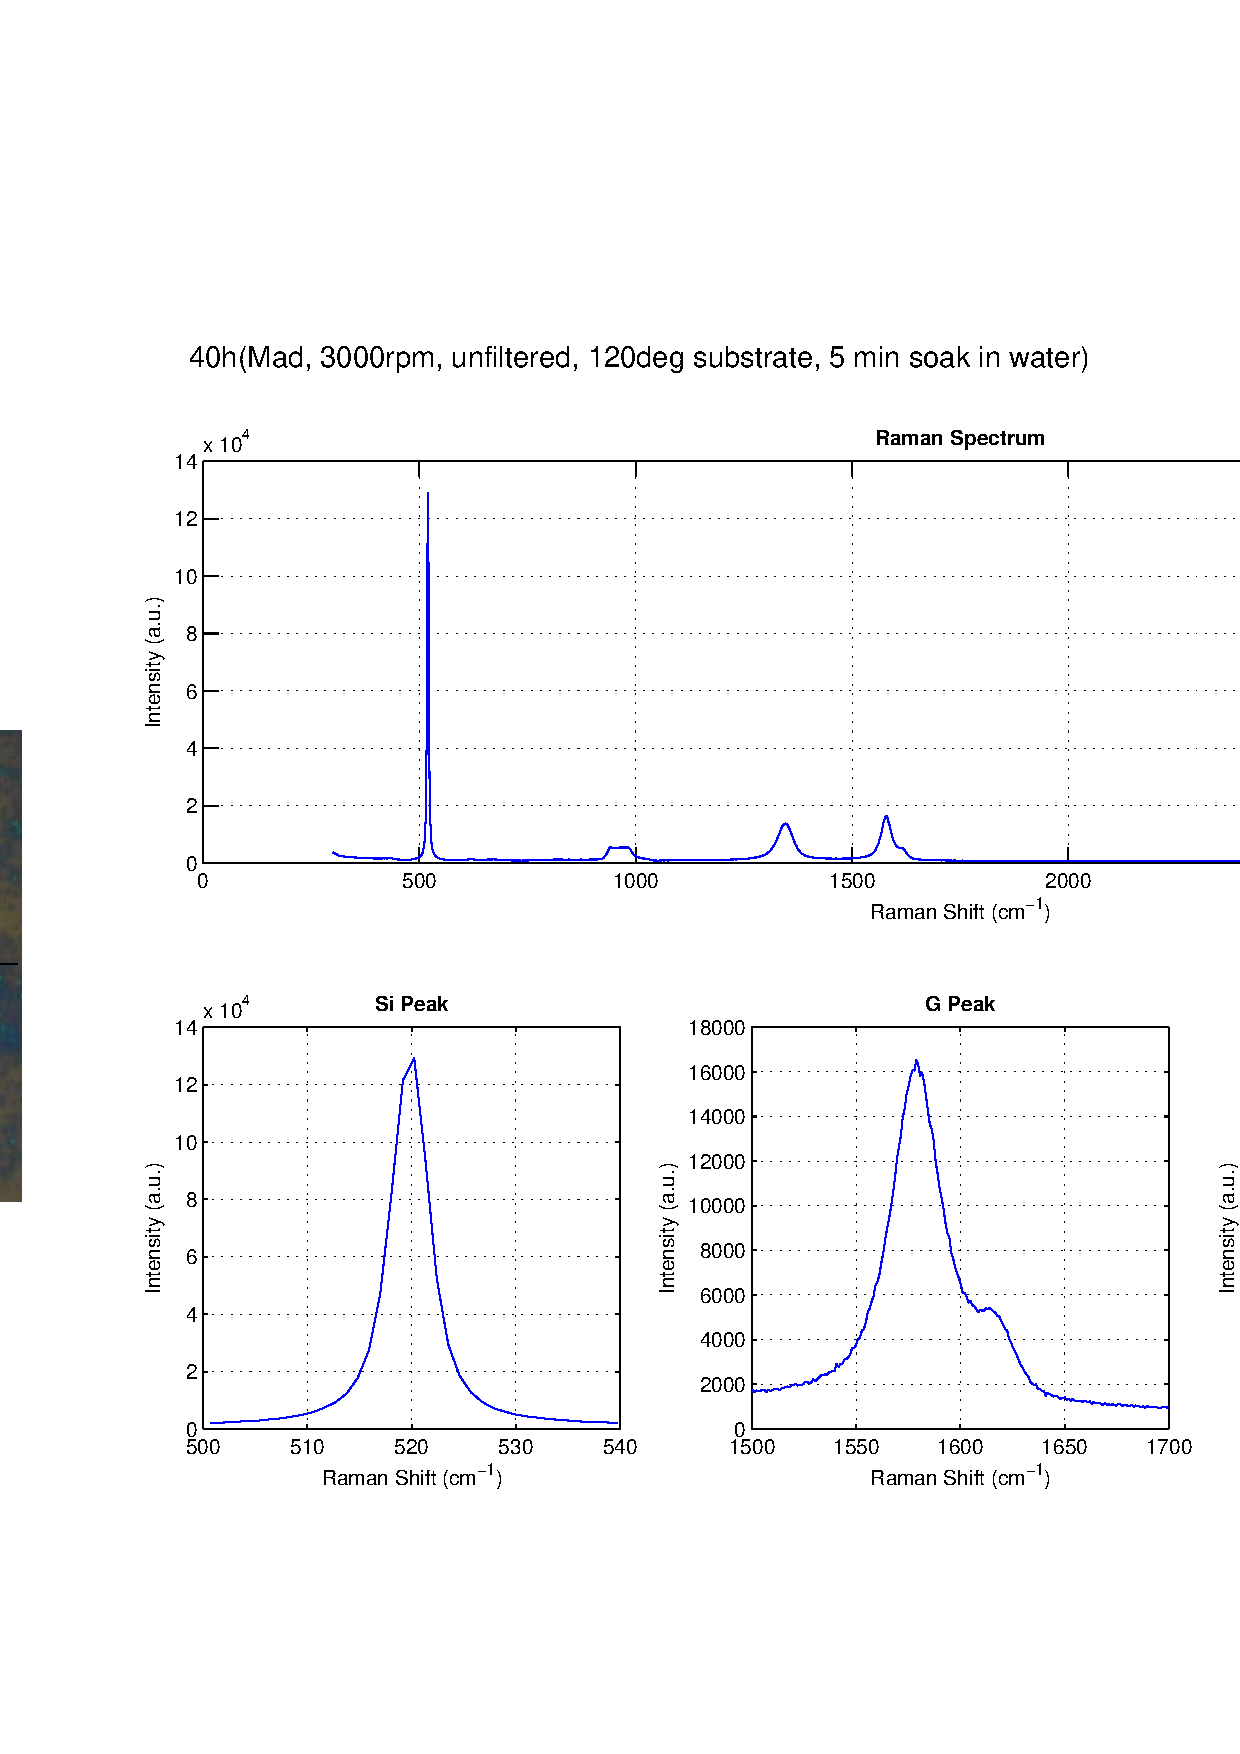
\includegraphics[width=1\textwidth]{figures/best.png}
		\caption[Clearest raman spectrum found for graphene.]{Raman spectrum of sample containing Madagascan graphite sonicated for 40 hours, centrifuged at 3000rpm, sprayed onto a substrate and soaked in water for 5 minutes. The spectrum clearly shows a G peak with intensity much smaller than the silicon peak, and a symmetrical 2D peak. The spectrum was generated using the script detailed in Appendix \ref{app:ramanratio}.}
		\label{fig:mad-sample}
	\end{figure}
	
	\begin{figure}
		\centering
		\includegraphics[width=1\textwidth]{figures/best-few-layer.png}
		\caption[Clearest raman spectrum found for few layer graphene.]{An example of a measured raman spectrum of few layer graphene from a sample containing Chinese graphite sonicated for 40 hours, sprayed onto a substrate and soaked in water for 5 minutes. The spectrum clearly shows a taller G peak than that seen for graphene, and an asymmetrical 2D peak. The spectrum was generated using the script detailed in Appendix \ref{app:ramanratio}.}
		\label{fig:best-few-layer}
	\end{figure}
	
	\begin{figure}
		\centering
		\includegraphics[width=1\textwidth]{figures/pristine.eps}
		\caption[Pristine graphene raman spectra.]{Raman spectra of pristine graphene samples chosen for their similarity with the expected raman spectrum of graphene. The silicon peak is omitted for scale.}
		\label{fig:pristine-raman}
	\end{figure}
	
	The ratio between the intensities of the G peak and the silicon peak was used to determine the number of layers present in each measurement. The script shown in Appendix \ref{app:ramanratio} was used to determine this ratio and display peaks in detail for analysis. To determine the number of layers our values were compared to past work performed by another undergraduate group at the centre for graphene science at Exeter University \cite{WillMoo}. These values were found using mechanical exfoliation of graphene and measuring the number of layers using the intensities of light from the flake and the substrate. This involves taking an optical micrograph of the flake and substrate under white light, and calculating $C = (I_f-I_s)/I_s\times100\%$ where $C$ is the relative shift of intensity of the flake ($I_f$) with respect to the intensity of the substrate ($I_s$). Step-like changes are visible with increasing optical contrast representing the number of graphene layers in a flake which are confirmed using raman spectroscopy (figure \ref{fig:contrast})\cite{Khrapach2012a}. These values were then compared to our measured values of the $I_G/I_{Si}$ ratio to determine the thickness of flakes. Figure \ref{fig:thickness-data}, shows measured values from a selection of our samples fitted to this data, and table \ref{tab:thickness-data} details the samples that successfully fit.
	
	\begin{figure}
		\centering
		\includegraphics[width=0.5\textwidth]{figures/contrast.png}
		\caption[Determination of thickness using optical contrast.]{The optical contrast of few layer graphene on glass. Contrast is calculated from optical micrographs of flakes under white light. Step-like changes are visible indicating the number of layers of flakes \cite{Khrapach2012a}.}
		\label{fig:contrast}
	\end{figure}
	
	\begin{figure}
		\centering
		\begin{subfigure}{1\textwidth}
			\centering
			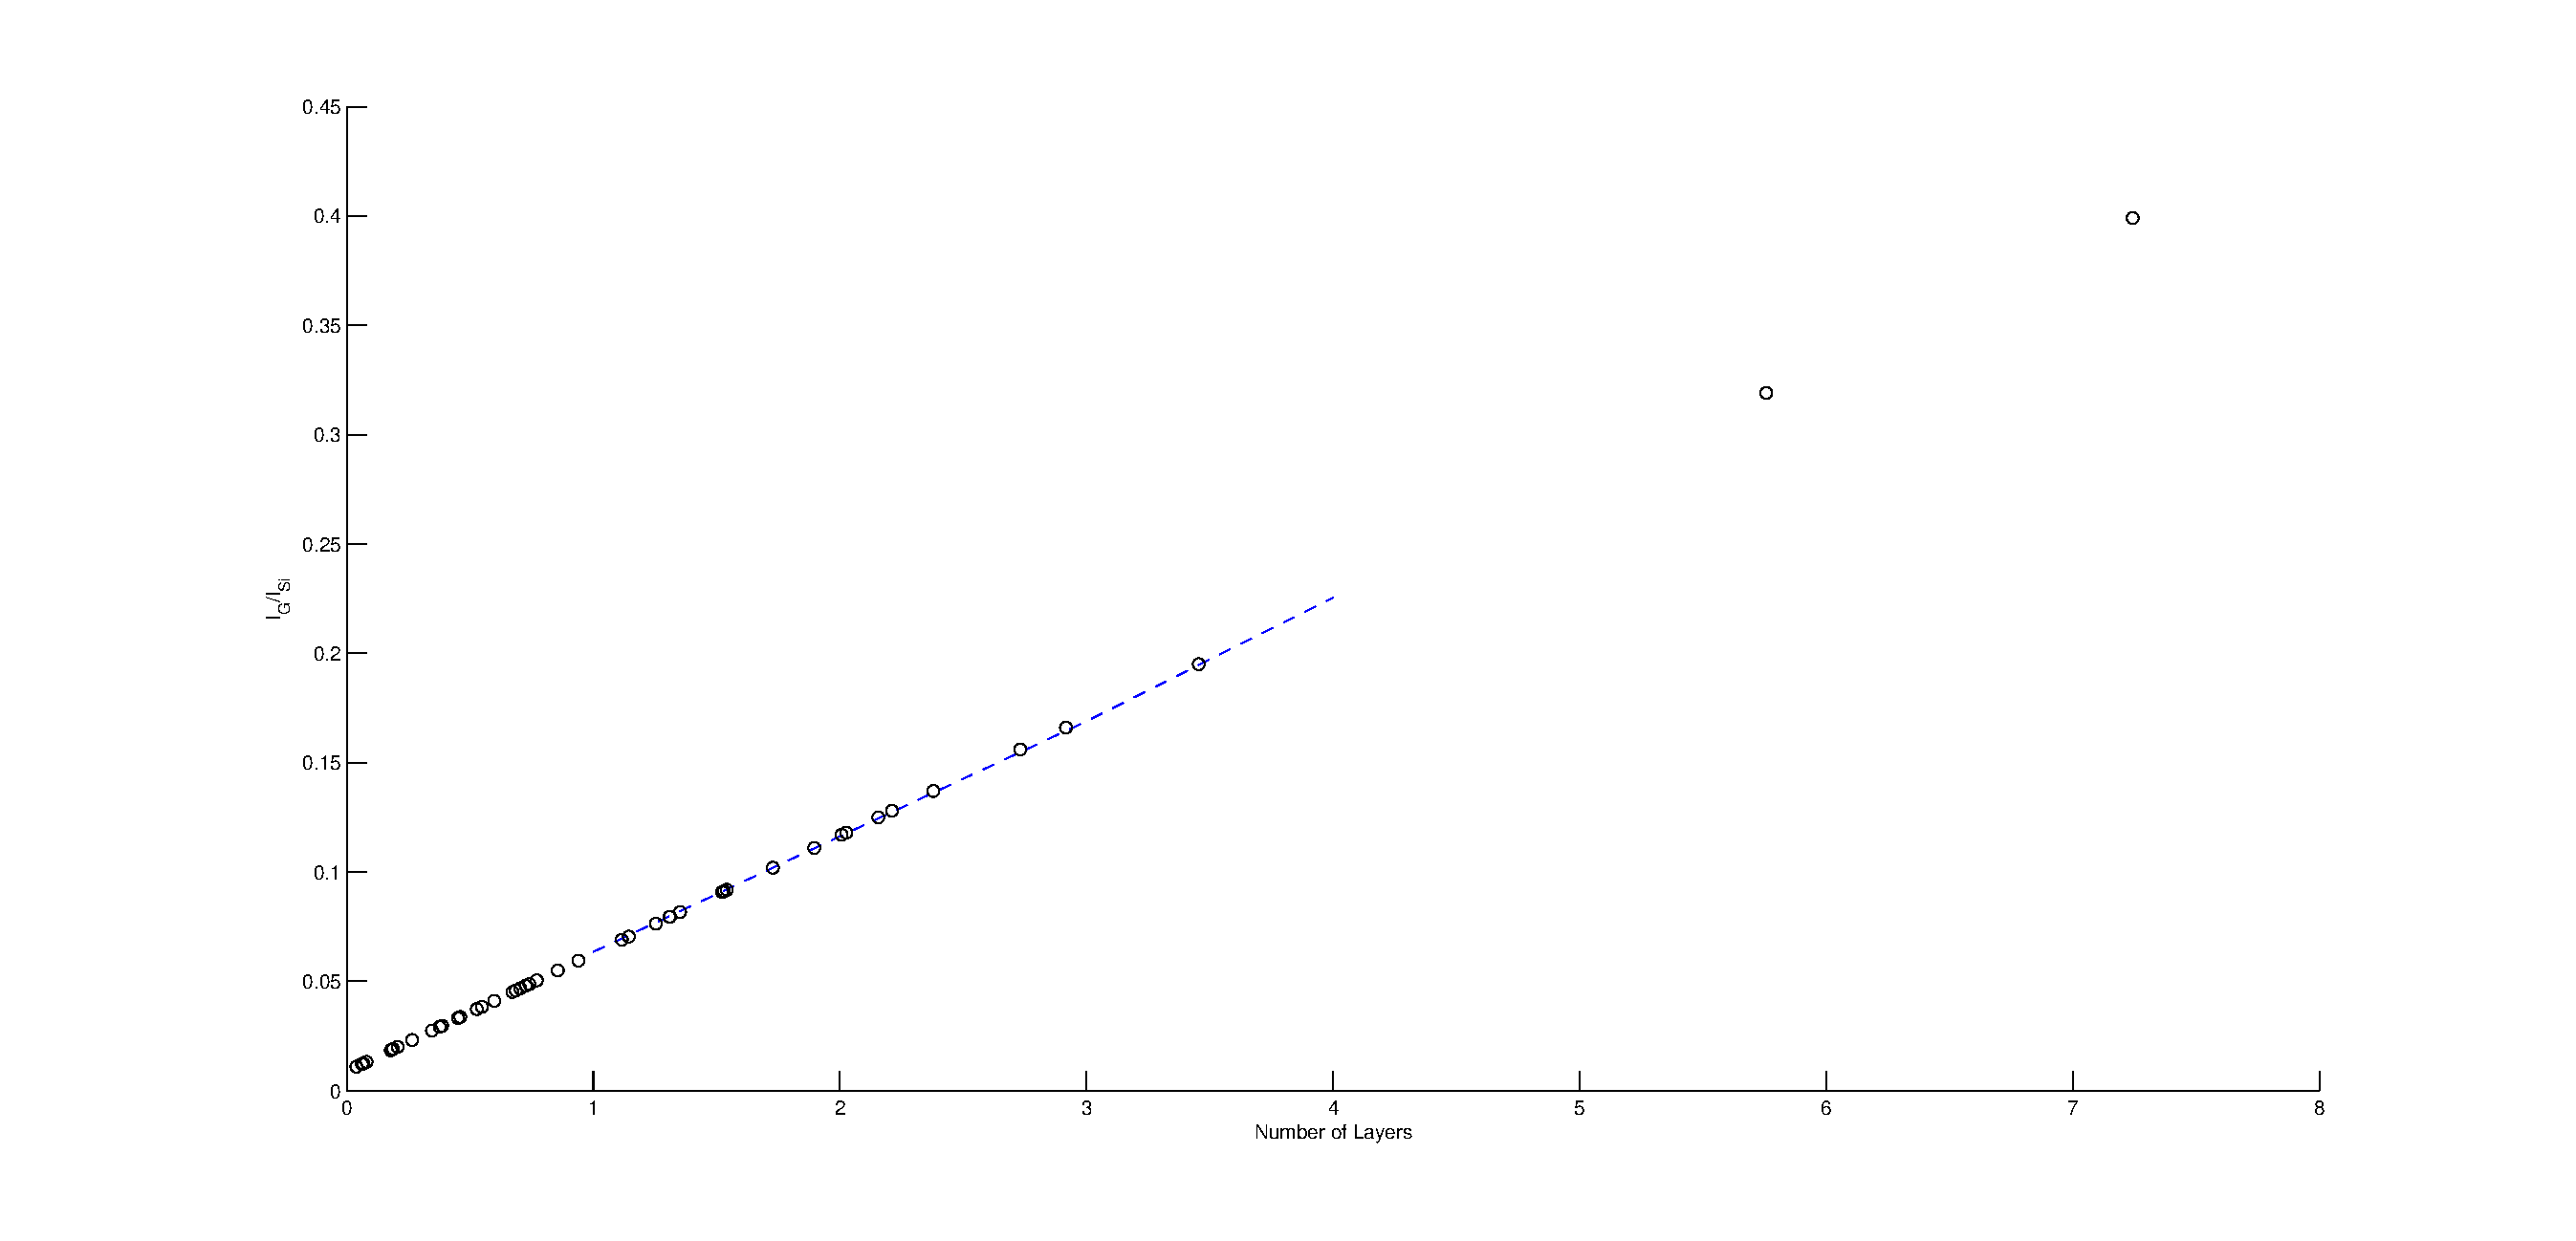
\includegraphics[width=\textwidth]{figures/thickness-data.eps}
			\label{fig:thickness-data-out}
		\end{subfigure}
		\begin{subfigure}{1\textwidth}
			\centering
			\includegraphics[width=\textwidth]{figures/thickness-data-zoom.eps}
			\label{fig:thickness-data-zoom}
		\end{subfigure}
		\caption[Determination of thickness using $I_G/I_{Si}$ ratio.]{Determination of thickness using $I_G/I_{Si}$ ratio. (Top) For samples with \textless 1 determined layers it is likely the intensity of the silicon peak has been artificially increased due to the laser spot being larger than the flake being measured. Samples with \textgreater 4 layers are likely thick graphite and are outside the capabilities of this method. (Bottom) Samples with layers determined by this method.}
		\label{fig:thickness-data}
	\end{figure}
	
	\begin{table}
		\begin{scriptsize}	
			\begin{tabularx}{\textwidth}{X X X X X}
				\hline
				$I_G/I_{Si}$ Ratio & Exfoliation Time & Graphite type & Centrifuge Speed & Intercalation \\
				\hline
				0.0705 & 40 hours & Sri Lankan & None & 8 hours VPI \\
				0.0764 & 40 hours & Madagascan & 3000rpm & \\
				0.0764 & 40 hours & Madagascan & 3000rpm & \\
				0.0794 & 40 hours & Madagascan & 3000rpm & 29 hours LPI \\
				0.0795 & 40 hours & Madagascan & 3000rpm & 29 hours LPI \\
				0.0817 & 40 hours & Madagascan & 3000rpm & 5 hours LPI\\
				0.0909 & 40 hours & Korean & None & \\
				0.0913 & 40 hours & Madagascan & 4000rpm & \\
				0.0919 & 30 hours & English & None & Simultaneous\\
				0.102 & 40 hours & Madagascan & None & \\
				0.111 & 40 hours & Madagascan & None & \\
				0.117 & 40 hours & Madagascan & 3000rpm & 13 hours LPI \\
				0.118 & 40 hours & Madagascan & 3000rpm & 13 hours LPI \\
				0.125 & 40 hours & Madagascan & 3000rpm & 29 hours LPI \\
				0.125 & 40 hours & Sri Lankan & None & \\
				0.128 & 40 hours & Madagascan & None & \\
				0.128 & 40 hours & Madagascan & None & \\
				0.137 & 40 hours & Madagascan & None & \\
				0.137 & 40 hours & Madagascan & 3000rpm & 29 hours LPI\\
				0.156 & 40 hours & Madagascan & 3000rpm & 13 hours LPI\\
				0.166 & 40 hours & Chinese & None & \\
				0.195 & 20 hours & English & None & Simultaneous \\
			\end{tabularx}
		\end{scriptsize}
		\caption[Samples with thickness determined by $I_G/I_{Si}$ ratio.]{Samples with thickness determined by $I_G/I_{Si}$ ratio.}
		\label{tab:thickness-data}
	\end{table}
	
	Previous studies suggest that this method is only effective to determine the thickness of flakes with up to four layers \cite{Khrapach2012a}. Many measurements of samples that gave raman spectra consistent with that of few layer graphene could not be fitted to this graph, giving a result of less than 1 layer of graphite. This is likely due to the fact that graphene flakes measured with the raman spectrometer were often smaller than the diameter of the laser spot. This would cause the silicon peak to be artificially larger, and the G peak to be artificially smaller than if the laser spot was covering only graphene. Therefore for smaller flakes (with a diameter of approximately $<1\mu$m) this technique of determining thickness was ineffective. Flakes that appeared to have more than 4 layers using this technique were likely thick graphite, with thicknesses outside of the capabilities of this method.
	
	For measurements that appear between two layers, it is likely the laser of the raman spectrometer is pointing over a region of flakes with varying thickness. For example if a measurement has an x-value of 1.4 on this plot, it is likely that the laser spot covers 60\% single layer graphene, and 40\% bilayer graphene.
	
	\subsection{Liquid-Phase Intercalation}
	In most cases a large proportion of iron chloride was used in comparison to the amount of graphite in a sample. This was to ensure there was enough iron chloride in the dispersion for intercalation to take place. However high concentrations of iron chloride made optical identification of flakes difficult since a large amount of residue was left over after deposition. Soaking with water after deposition to remove excess iron chloride was attempted. Substrates were soaked for only 1 second to prevent the water from encouraging deintercalation of flakes but still this caused most of the flakes to wash off the substrate, and any remaining flakes showed no sign of intercalation so this was not pursued further. When flakes were visible underneath the iron chloride through an optical microscope they were found to be more brown in colour than before intercalation.
	
	%Comparison pictures
	%Picture - increasing concentration
	%Picture - increasing time
	
	Simultaneous LPE and LPI only yielded negative results. Not only was no intercalation observed, but only thick graphite flakes were observed using raman spectroscopy after centrifugation. The diameter of these flakes decreased as sonication time was increased. This suggests the introduction of iron chloride may have prevented the separation of graphene layers, whilst lateral breakup of flakes still took place.
	
	%Picture - simultaneous raman, comment not much change and low peak intensity.
	
	%Best results came from & reference of grouped graph.
	Raman spectra of samples from the LPI process with the clearest peaks resembling the expected raman spectrum of intercalated graphene came from samples of Madagascan graphite sonicated for 40 hours, centrifuged at 3000rpm for 90 minutes, then sonicated with 5g/100ml of FeCl$_3$ for 7 hours at $80^{\circ}$C and sprayed onto a substrate heated to $120^{\circ}$C. A raman spectrum from this sample can be seen in figure \ref{fig:best-interc}. However raman spectra from this sample do not show clear splitting of the G peak in G$_1$ and G$_2$ peaks, but show a clear broadening of the G peak suggesting partial intercalation of flakes may have taken place.
	
	In order to compare this data with methods used in previous studies \cite{Khrapach2012a} a selection of samples containing graphene and few layer graphene were selected containing different types of graphite to be used in a vapour-phase intercalation process. Samples were annealed at $250^{\circ}$C for 3 hours and again at $400^{\circ}$C for 3 hours to remove any water molecules in the sample. Vapour-phase intercalation was then performed for 8 hours. 
	
	\begin{figure}
		\centering
		\includegraphics[width=1\textwidth]{figures/best-interc.png}
		\caption[Clearest raman spectrum found for intercalated graphene.]{G peak of raman spectrum of sample containing Madagascan graphite sonicated for 40 hours, centrifuged at 3000rpm for 90 minutes, then sonicated with 5g/100ml of FeCl$_3$ for 7 hours at $80^{\circ}$C and sprayed onto a substrate heated to $120^{\circ}$C. There is a clear indication of broadening of the peak where separate G$_1$ and G$_2$ peaks are expected. This suggests the sample has been partially intercalated. The expected locations of the G ($1580\text{cm}^{-1}$), G$_1$ ($1612\text{cm}^{-1}$) and G$_2$ ($1625\text{cm}^{-1}$) peaks are labelled.}
		\label{fig:best-interc}
	\end{figure}
	
	For thin flakes, only very low intensity peaks were found near the expected locations of the G$_1$ and G$_2$ peaks on these samples. However evidence for intercalation was found in thick graphite flakes, with a clear splitting of the G peak observed over the expected location of the G$_1$ peak (figure \ref{fig:graphite-vpi}). If thick flakes have been intercalated but thin flakes on the same sample have not, this may suggest that thin flakes with small diameters are too small to remain stable after intercalation has taken place, and the iron chloride does not stay between the graphene layers. Figure \ref{fig:intercalated} shows a collection of measurements from various samples containing thin flakes intercalated through LPI and VPI showing broadening of the G peak.
	
	\begin{figure}
		\centering
		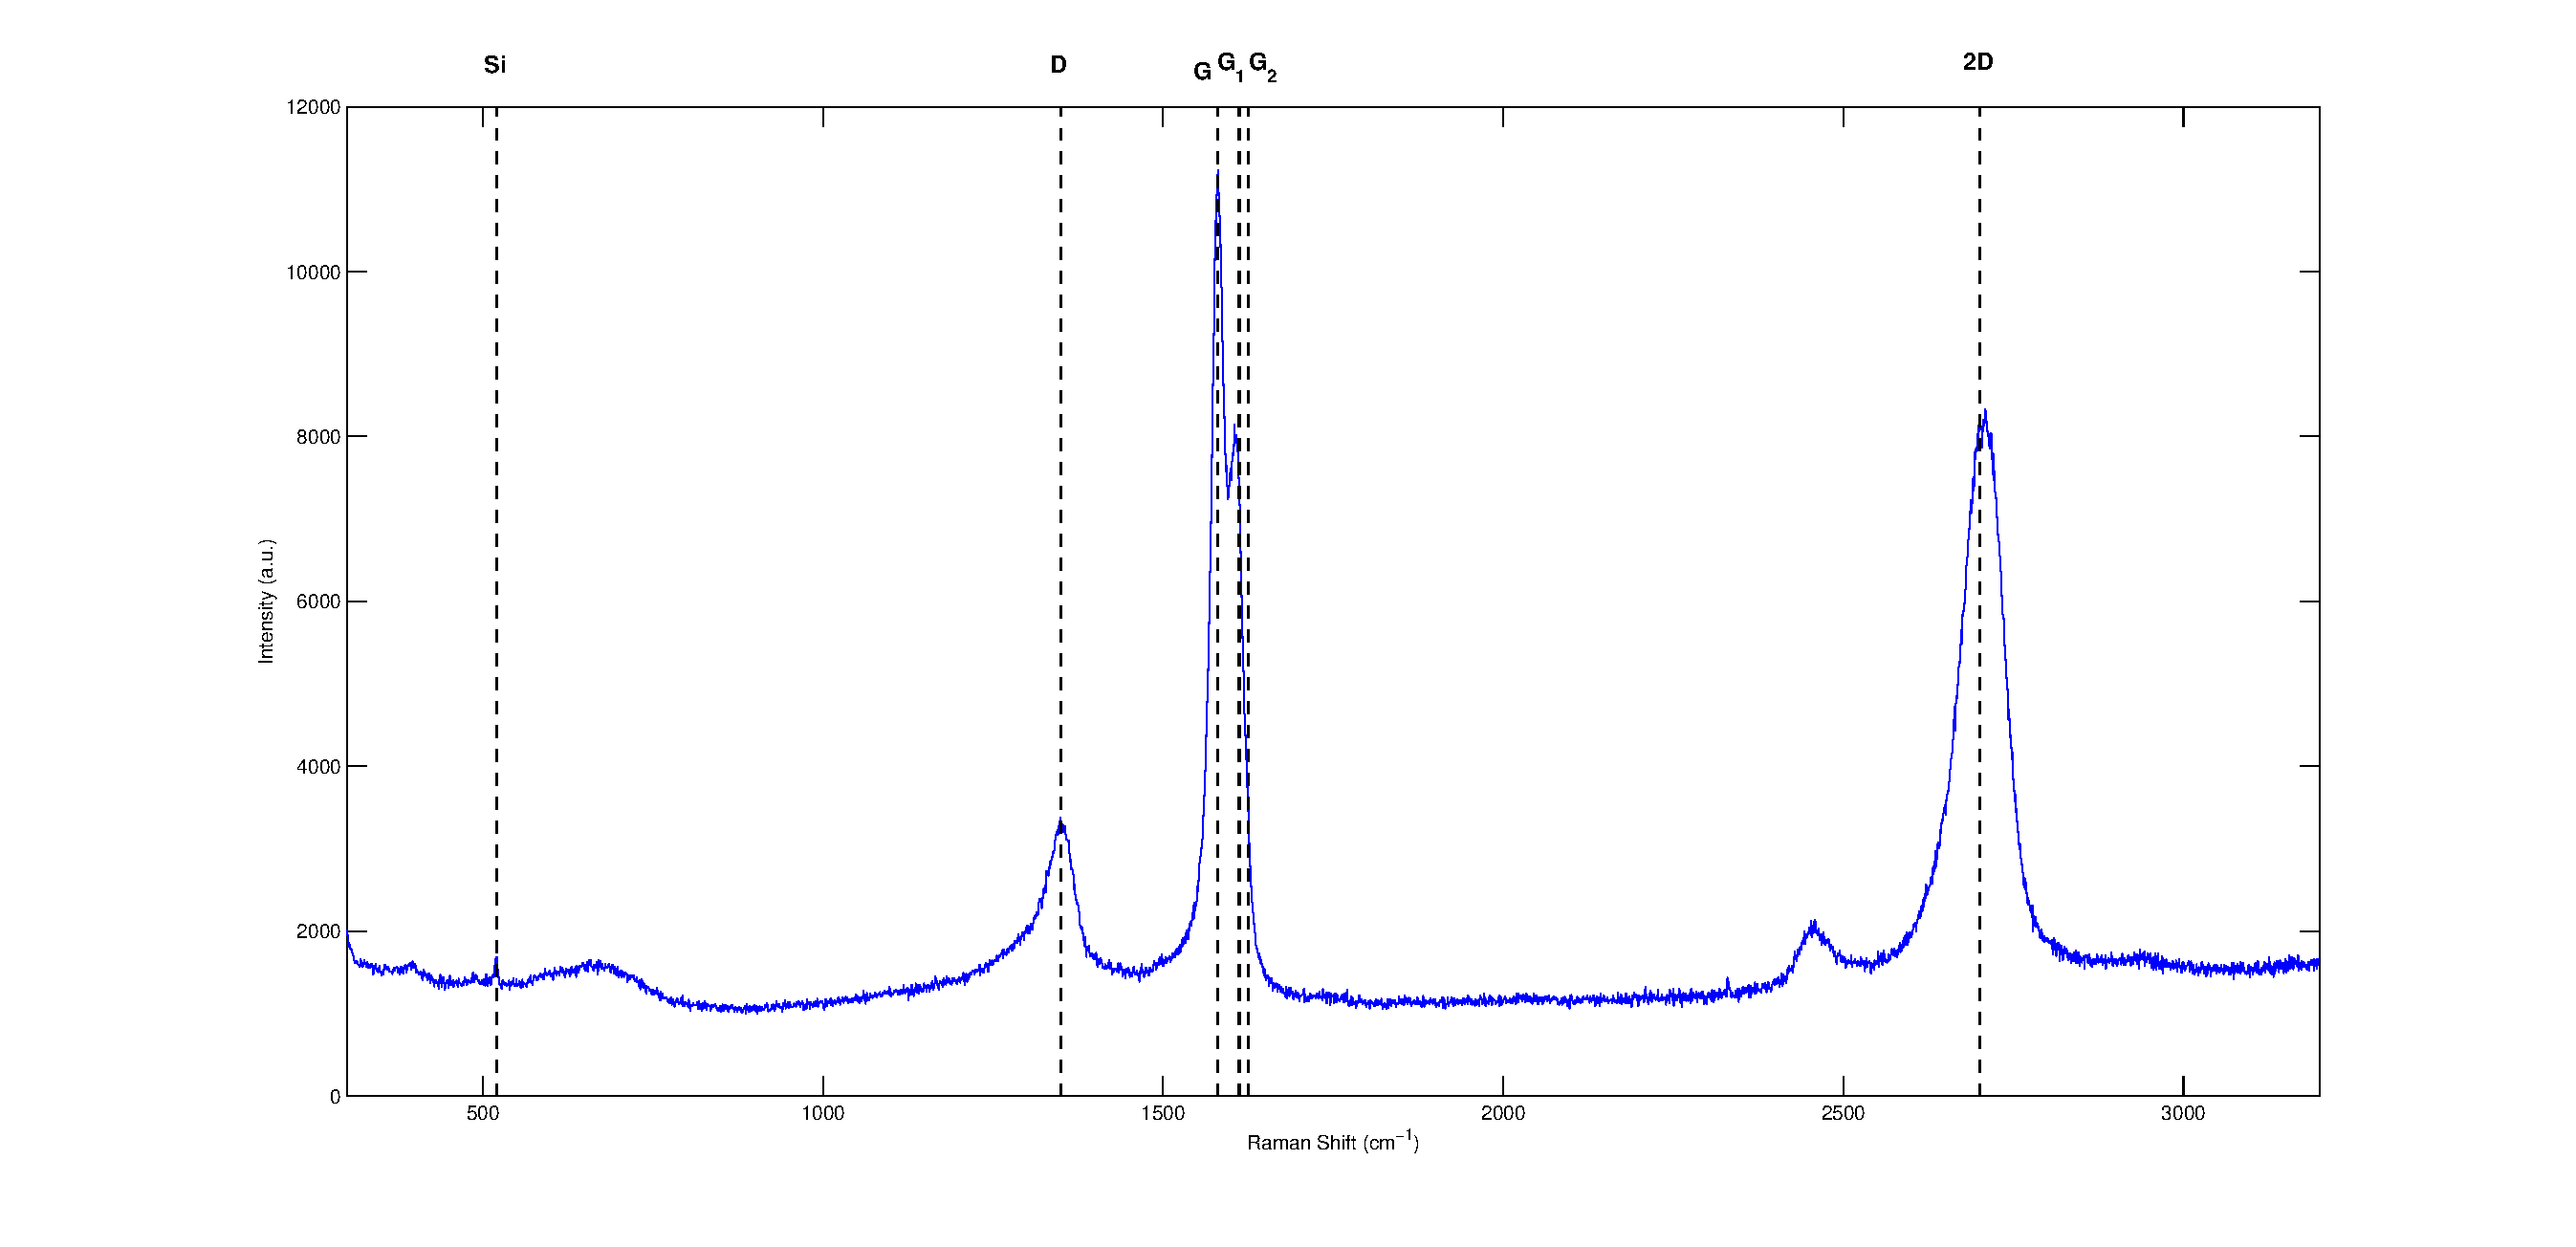
\includegraphics[width=1\textwidth]{figures/graphite-vpi.eps}
		\caption[Graphite intercalated by vapour phase.]{Raman spectra of a thick flake of korean graphite exfoliated from 40 hours of LPE, sprayed onto substrate and intercalated by vapour-phase. The low intensity of the silicon peak in comparison to the G peak shows that this is thick graphite. A peak can be seen where the G$_1$ peak is expected, and the 2D peak is symmetrical suggesting intercalation has occurred.}
		\label{fig:graphite-vpi}
	\end{figure}
	
	%Add new graph for intercalations. Does it have splitting mentioned above?
	\begin{figure}
		\centering
		\begin{subfigure}{1\textwidth}
			\centering
			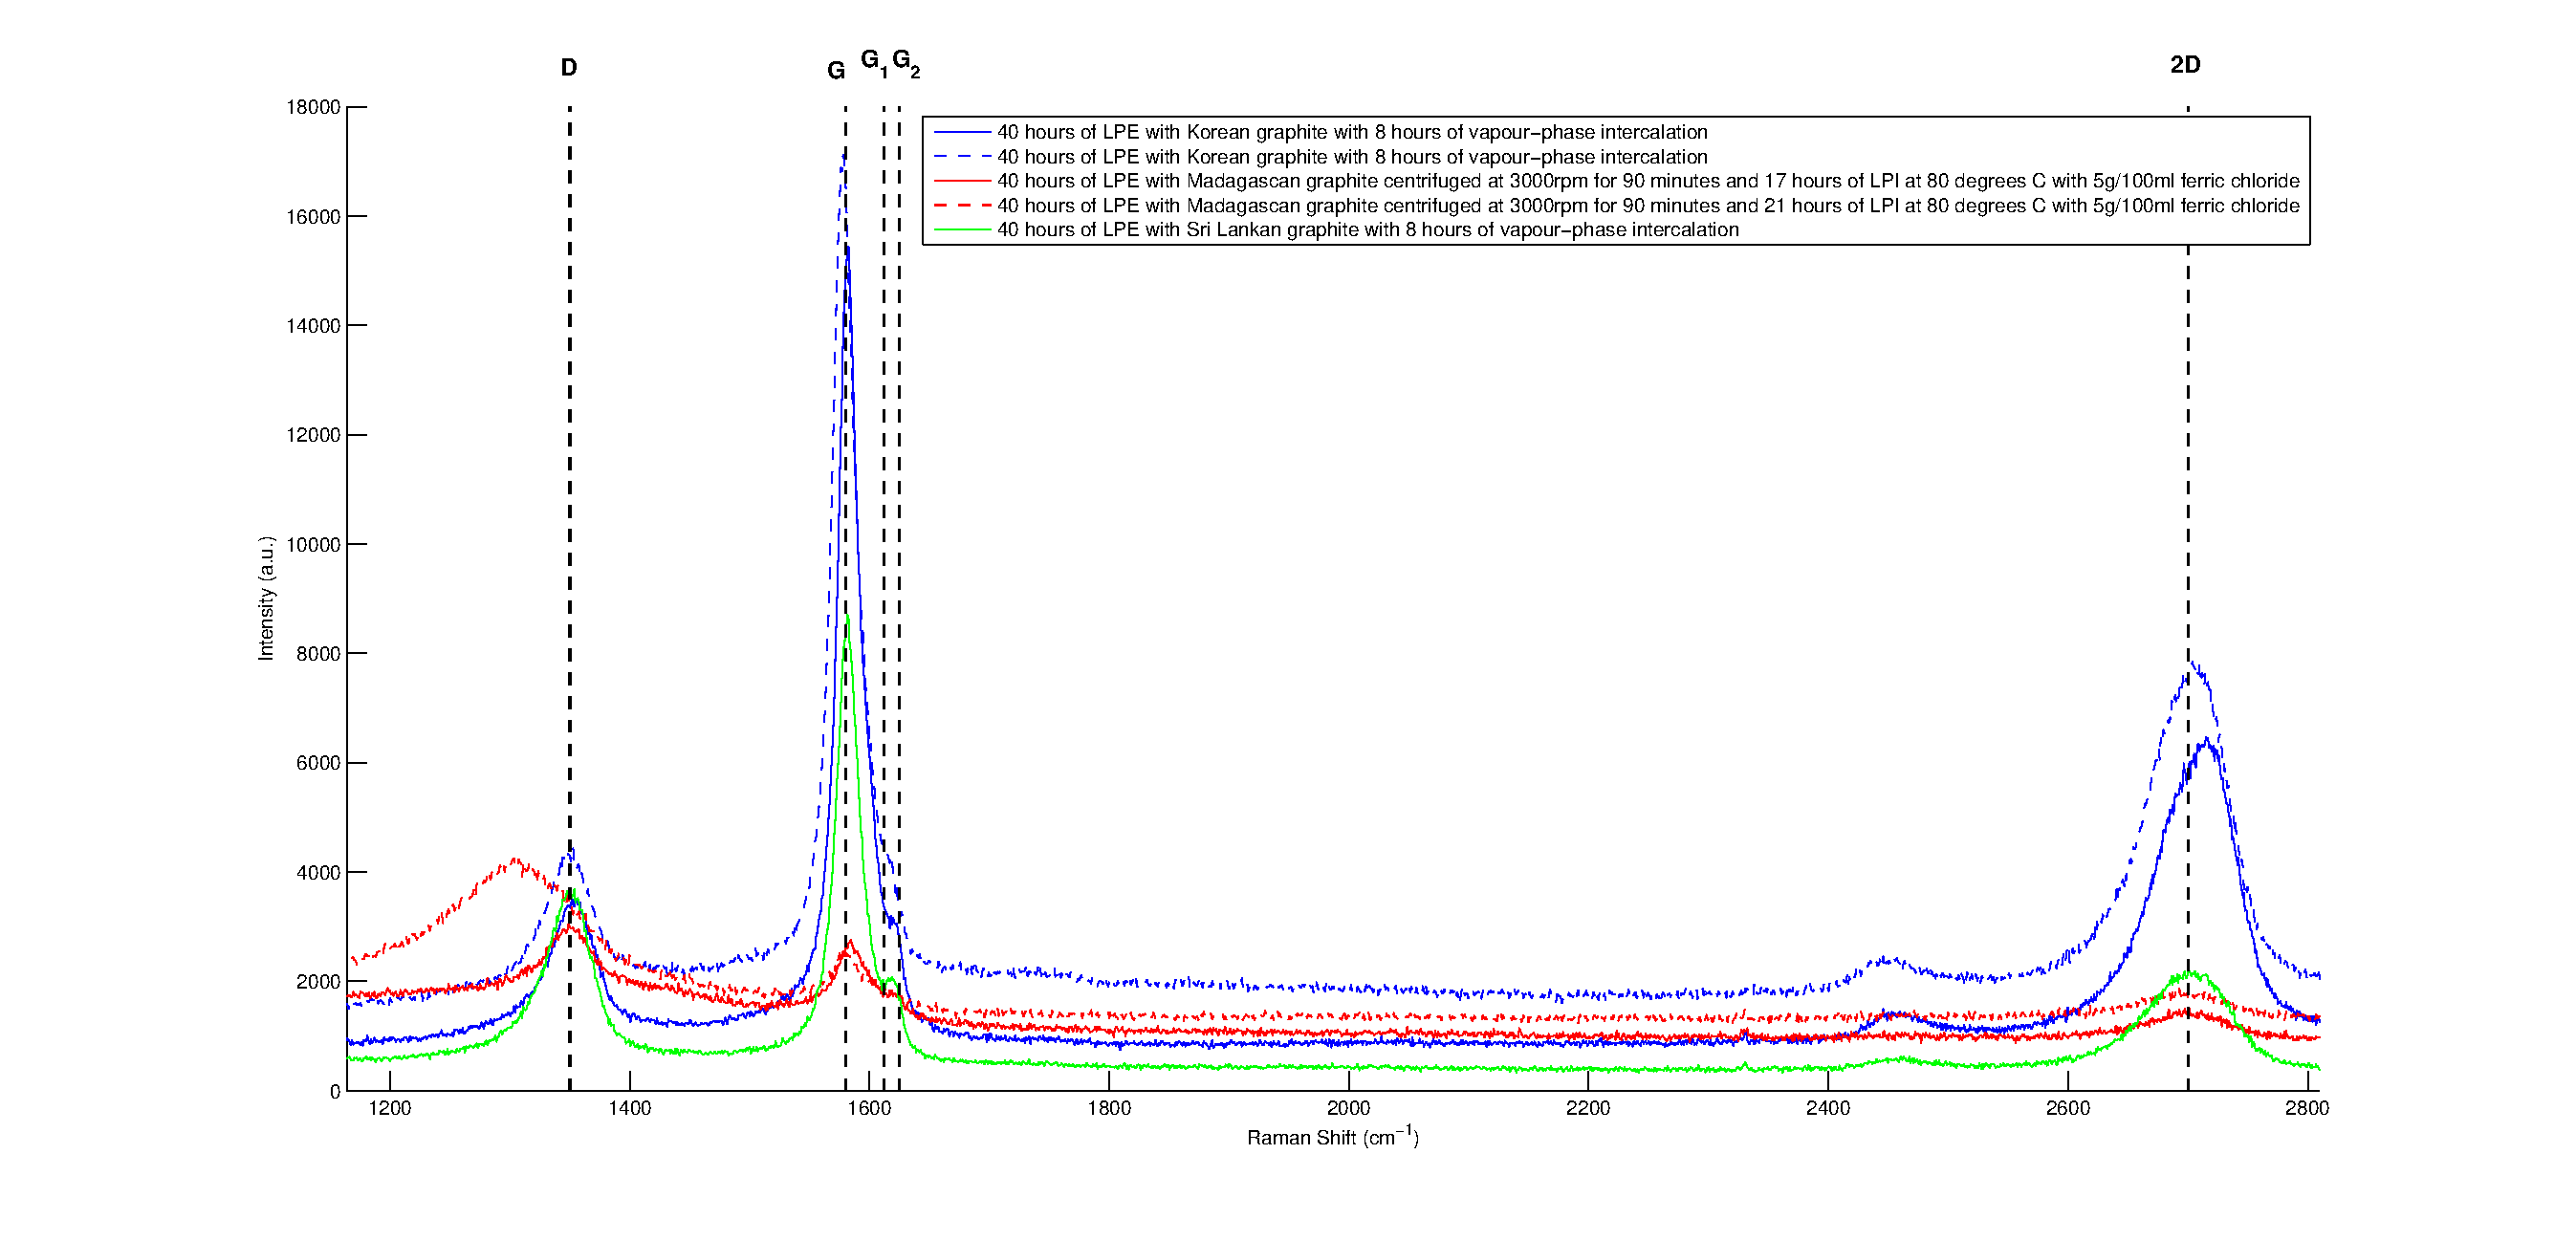
\includegraphics[width=\textwidth]{figures/intercalated.eps}
			\caption{Raman spectra (silicon peak omitted for scale).}
			\label{fig:intercalated-all}
		\end{subfigure}
		\begin{subfigure}{1\textwidth}
			\centering
			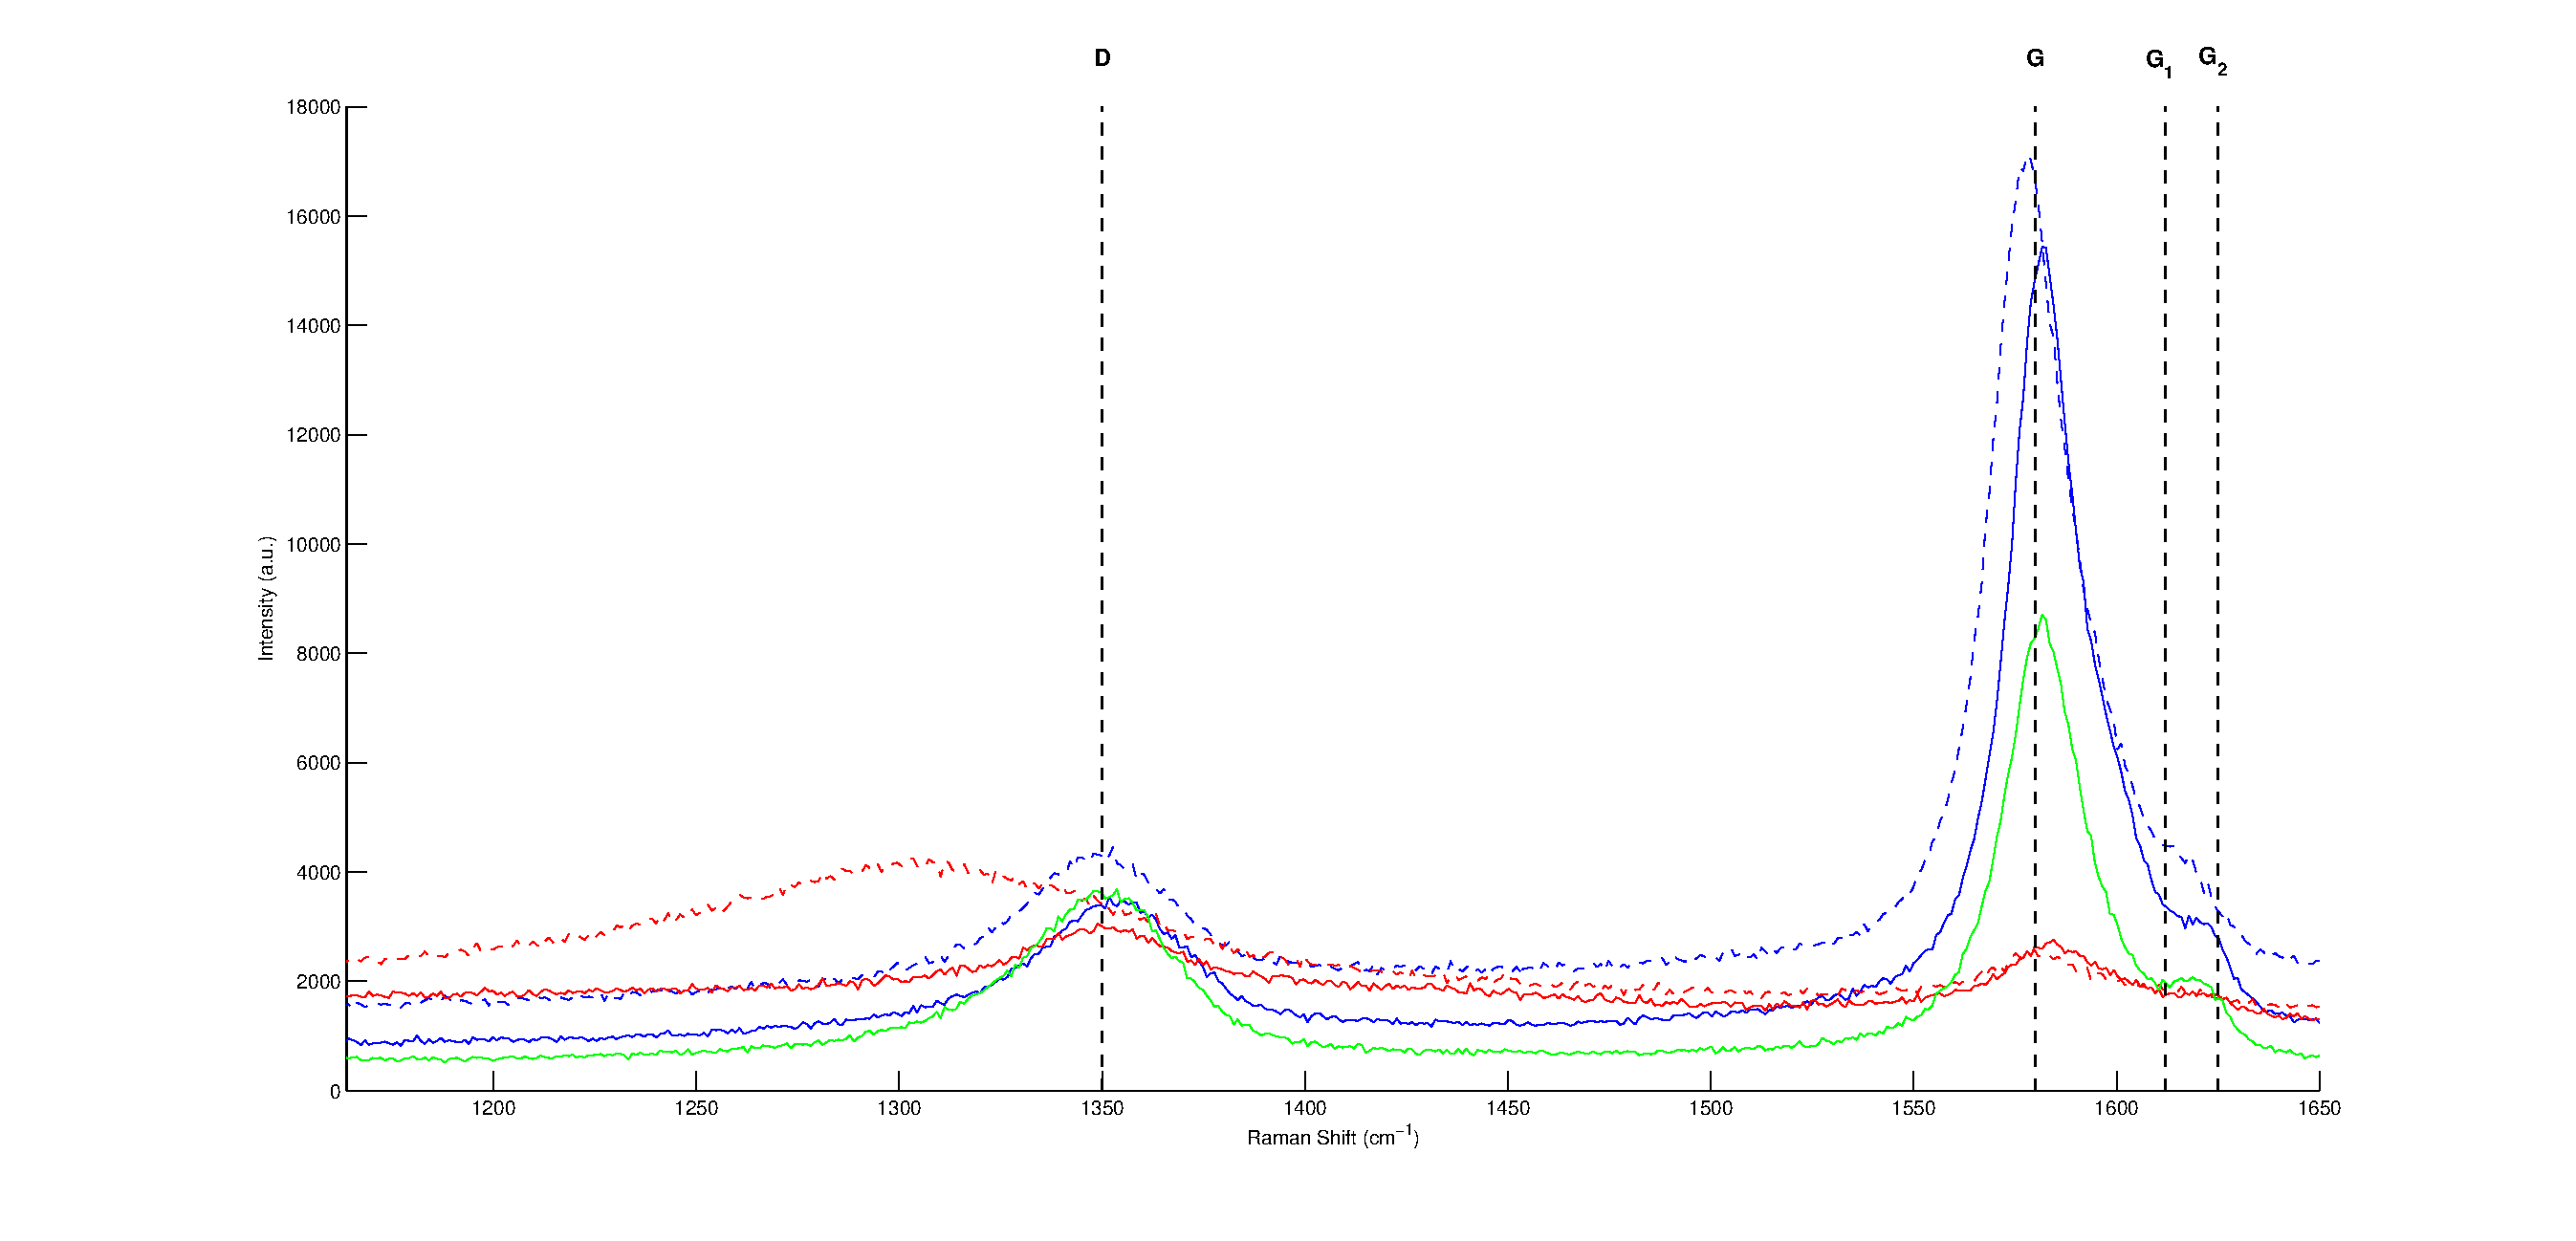
\includegraphics[width=\textwidth]{figures/intercalated-DG.eps}
			\caption{The D and G peaks.}
			\label{fig:intercalated-DG}
		\end{subfigure}
		\caption[Raman spectra of intercalation samples.]{Raman spectra of intercalation samples chosen for their similarity with the expected raman spectrum of intercalated graphene. The silicon peak is omitted for scale, and the expected location of the G ($1580\text{cm}^{-1}$), G$_1$ ($1612\text{cm}^{-1}$) and G$_2$ ($1625\text{cm}^{-1}$) peaks are shown.}
		\label{fig:intercalated}
	\end{figure}
	
	\subsection{Limitations}
	
	%Broadening of G-peak, but no true splitting.
	There are some limitations to this data. Evidence of intercalation having taken place requires a splitting of the G peak into G$_1$ ($1612\text{cm}^{-1}$) and G$_2$ ($1625\text{cm}^{-1}$) peaks. Clearly this has not taken place and only a broadening of the G peak was observed in the best cases of LPI. This is not expected to take place for any reason other than intercalation, but it is possible that this had been caused by defects in the sample or errors in the measurement.
	
	%Possibly distiorted by D'
	There is another raman peak present in our samples known as the D' peak ($1620\text{cm}^{-1}$) \cite{Vidano1981}, situated very close to the G peak. This peak is due to interactions similar to that in the D peak but further from the $K$ point and is therefore much less likely to occur \cite{Thomsen2000}. This could contribute to the broadening of the G peak observed in intercalation samples. However the peak can also be seen on raman spectra measured for pristine graphene in figure \ref{fig:pristine-raman} and is clearly much lower in intensity than the G peak.
	
	\begin{figure}
		\centering
		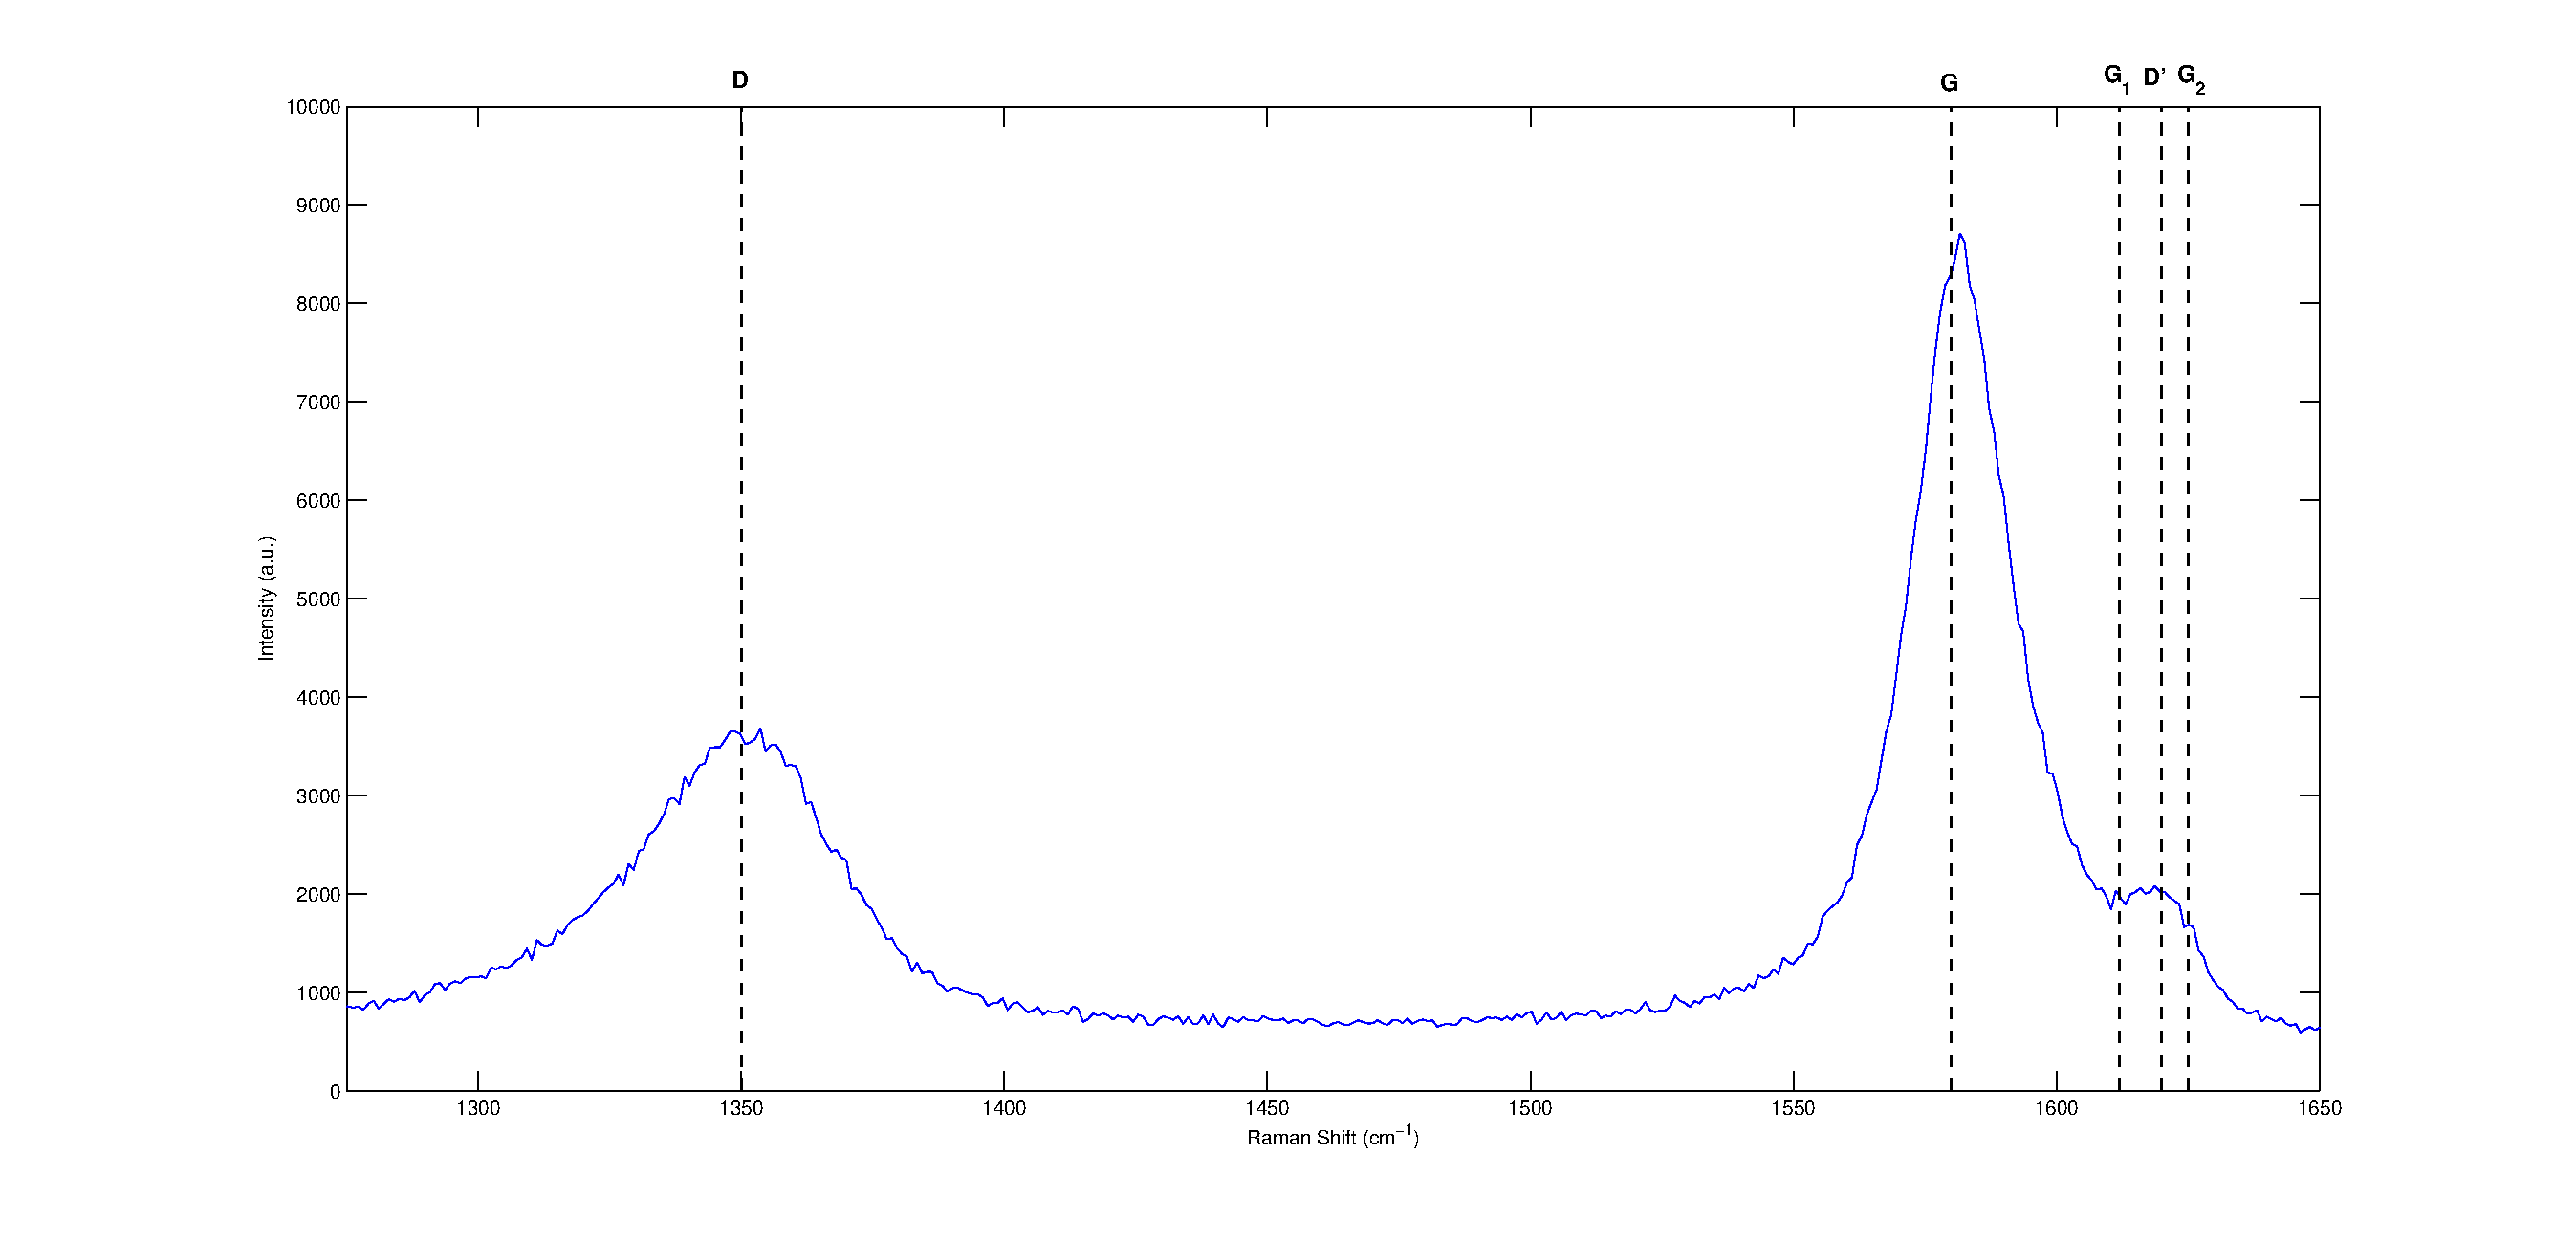
\includegraphics[width=1\textwidth]{figures/d-prime.eps}
		\caption[Analysis of the D' raman peak.]{Part of the raman spectrum of a thin flake of Sri Lankan graphite exfoliated for 40 hours and intercalated through vapour-phase. The peak to the right of the G peak aligns to the expected location of the D' peak rather than G$_1$ or G$_2$. This acts as an indication that the flake is not partially intercalated as it may initially appear.}
		\label{fig:d-prime}
	\end{figure}
	
	Some samples measured which may initially appear to be partially intercalated due to a splitting of the G peak into G$_1$ or G$_2$, are likely to be split as a result of this D' peak. For example in figure \ref{fig:d-prime} we can see one of the measurements shown in figure \ref{fig:intercalated}, which has a small peak situated to the right of the G peak. When the expected location of the D' peak is displayed alongside the G$_1$ and G$_2$ peaks, it is clear that this is most likely resulting from the D' process and does not represent intercalation. In many samples it is very difficult to tell which process a peak may result from. In figure \ref{fig:d-prime} the D' peak has approximately half the intensity of the D peak. Therefore if a suspected G$_1$ or G$_2$ peak is approximately half the intensity of the D peak, this may indicate that it is in fact a D' peak and intercalation has not taken place.
	
	%Saw many other strange raman graphs?
	
	Therefore we must consider the possibility that all small flakes that show a shoulder on the G peak indicating partial intercalation, are in fact showing a larger than normal D' peak, and are not intercalated at all. Even if the small flakes are partially intercalated we saw none that we fully intercalated even after the accepted vapour-phase intercalation process \cite{Khrapach2012a}. However after this process we saw strong signs of intercalation in thick graphitic flakes.
	
	These results suggest that graphene flakes exfoliated through the process of LPE are too small to remain stable when intercalated with iron chloride. This means that if improvements are made to the liquid-phase exfoliation process to created graphene flakes with a larger diameter, intercalation may remain stable. This could also be possible if the LPE process stays the same, but a type of graphite is found which exfoliated larger flakes. Once this has been achieved, and flakes remain intercalated after vapour-phase intercalation, the vapour-phase intercalation process can be investigated further.
			
	\newpage
	\section{Conclusions}
	
	%Raman spectra from LPE suggest liquid exfoliation of graphene haas been acheived.
	The aim of this project was to create graphexeter in liquid dispersion for spraying on to substrates. The simplest and cheapest method found for doing this on a large scale was to first create graphene in liquid dispersion through a method of liquid-phase exfoliation and then intercalate this in liquid-phase to create graphexeter.
	
	Liquid-phase exfoliation of graphene was performed by sonicating graphite flakes in an aqueous dispersion. Raman spectra of samples sonicated for 40 hours and centrifuged to filter out thicker flakes (figure \ref{fig:pristine-raman}) were consistent with that expected for single layer and few layer graphene (figure \ref{fig:raman}). From this data we can say that liquid-phase exfoliation of few layer and single layer graphene has been achieved. However finer control over the number of layers of graphene present in flakes will require further study.
	
	%Lack of flake coverage/large flakes causes laser spot to be bigger than flakes making number of layers difficult to determine.
	A simple method of precisely quantifying the number of layers present in a flake of few layer graphene was performed using the raman spectra of the graphene flake and taking the ratio of intensities between the silicon peak and the G peak using the script detailed in Appendix \ref{app:ramanratio}. However this method was only valid if the laser spot of the raman spectrometer covered only the graphene to be measured and no bare substrate, as this would artificially raise the intensity of the silicon peak and lower the value of the ratio. An increased density of flakes present on the substrate, or larger flakes would allow this method to be used more often to determine the number of layers present in a measurement.
	
	%Liquid phase intercalation showed broadening of the G peak acoss expected locations for the G1 and G2 peaks. Broadening of the G peak is not expected to occur for other reasons suggesting partial intercalation has taken place.
	Liquid-phase intercalation of graphene to create graphexeter was performed by dispersing iron chloride in samples and sonicating further. Raman spectra of intercalation samples sonicated for over 7 hours and sprayed onto substrates showed a broadening of the G peak (figure \ref{fig:intercalated}) across the locations of the G$_1$ and G$_2$ peaks that are expected for intercalated graphite (figure \ref{fig:raman}). This data suggests partial intercalation of flakes may have been achieved. Other possibilities for this broadening being observed are discussed, including the presence of the D' peak in between G$_1$ and G$_2$.
	
	Vapour-phase intercalation was also performed, with data in figure \ref{fig:intercalated} showing that intercalation has taken place for thick graphite flakes. However for small thin flakes, similar results to those of liquid-phase intercalation are seen. This suggests that flakes with smaller diameter (approximately $\le 1\mu$m) are not stable after intercalation, and iron chloride does not remain between the graphene layers. 
	
	%Future work
	It is concluded that future work is required for liquid-phase intercalation to create thin graphene flakes with larger diameters that will remain stable after intercalation. This could be done by finding a type of graphite more susceptible to this exfoliation process, or by finding different solvents or surfactants that lower the energy required for exfoliation further.
	
	Liquid-phase intercalation could be improved by using higher temperatures or by performing processes for longer. Intercalation in vapour-phase is performed at temperatures up to $360^{\circ}$C \cite{Khrapach2012a}, whereas our liquid-phase processes were performed at $80^{\circ}$C as this was the maximum temperature our equipment would allow. At the time of writing, a machine was on order that would stir the dispersion using a magnetic stirrer, whilst heating up to $300^{\circ}$C. This would greatly increase the energy provided for intercalation, and prevent subsequent lateral breakup of flakes that would decrease their diameter. This could also help in the determination of the number of layers in a graphene sample using the $I_G/I_{Si}$ ratio of raman spectra, since this method requires flakes (or collections of flakes) to be larger than the laser spot of the raman spectrometer.
	
	To improve the coverage of graphene on the substrate, either a higher concentration of flakes in dispersion is required, or a higher number of spray coats. A higher density of flakes would allow for a continuous electrical channel across the substrate and would allow for electrical characterisation of samples to be performed on a macroscopic scale without the use of electron-beam lithography.
	
	The electrical characteristics of samples could be measured by creating transistor-like structures, with which charge transport parameters such as the mobility of electrons and the magnetic field and temperature dependance of resistance could be measured \cite{Kim2011,Ye2011}.
	
	\newpage
	\begin{appendices}
		\section{Script For Calculating Raman $I_G/I_{Si}$ Ratio and Displaying Raman Spectrum}
		\label{app:ramanratio}
		\lstinputlisting[language=Matlab,
						tabsize=2,
						breaklines=true,
						numbers=left,
						basicstyle=\footnotesize,
						title=ramanratio.m]{files/ramanratio.m}
						
		\newpage
		%\section{Table of Samples Tested}
	\end{appendices}
	
	\newpage
	\bibliographystyle{unsrt}
	\bibliography{refs,willmoo}{}
	
\end{document}

%TODO - 

%Add new types of graphite to the list of ones tested.
%Create new pristine plot with new Grpahene data.
%Add samples to thickness data graph.
%Add info in vapor-phase
%Add raman data for vapor phase

%Add extra references